
\documentclass{article}
\usepackage{jim,amsmath}
\usepackage[utf8]{inputenc}
\usepackage[francais]{babel}
\usepackage[T1]{fontenc}

\usepackage{xcolor,graphicx}
\usepackage{comment}
\usepackage{verbatim}


\newenvironment{gmncode}	{\vspace{-2mm}\small\verbatim}{\endverbatim\vspace{-2mm}}
%\newenvironment{code}  		{\fontfamily{pnc}\selectfont}{}

\newcommand{\guido}			{\textsc{Guido}}
\newcommand{\exemple}		{\vspace{2mm}\hspace*{-6mm}\textsc{Exemple}}

\title{\centering Extension de Guido aux notations contemporaines}

%\date{ Février - décembre 2013}

\oneauthor
 {Camille Le Roi, Colas Decron, Dominique Fober} {
 Grame - Centre national de création musicale \\ 
\{cleroi, decron, fober\}@grame.fr
 }

%\threeauthors
%  {Camille Le Roi} {Grame \\ cleroi@grame.fr}
%  {Colas Decron} 	{Grame \\ cdecron@grame.fr}
%  {Dominique Fober} {Grame \\ fober@grame.fr}

\begin{document}

\selectlanguage{french}

\maketitle

\begin{abstract}

Le projet \guido\ regroupe à la fois un format textuel de description de partitions musicales, un moteur de rendu basé sur ce format, et une librairie qui fournit aux développeurs d'applications, un support de haut niveau pour l'ensemble des services liés au format \guido\ et à son rendu sous forme graphique. 
De base, le projet \guido\ traite de la notation traditionnelle de la musique occidentale. Le projet a été récement étendu, tant du point de vue format que du point de vue rendu, pour adresser également les besoins les plus courants de la musique contemporaine. Cet article présente ces extensions et montre comment les choix de design fournissent à l'utilisateur, une large palette de solutions pour la notation de la musique. 

%La librairie \guido\ offre un grand nombre de symboles musicaux correspondant aux plus larges besoins de l'écriture musicale. Elle fournit un moteur de rendu de partitions embarquable dans d'autres applications. Dans une volonté d'étendre cette librairie à la musique contemporaine, nous avons implémenté un ensemble de nouvelles notations jusqu'à présent pas, ou très sommairement, implémentées. L'objectif était de répondre aux demandes des compositeurs en ajoutant certaines notations de la manière la plus adaptée à l'écriture musicale, tout en laissant une large liberté à l'utilisateur.

\end{abstract}

%%%%%%%%%%%%%%%%%%% INTRODUCTION %%%%%%%%%%%%%%%%%%%%

\section{Introduction}\label{sec:introduction}

% format
% librairie
% compos
% état de l'art de la notation contemporaine
% pb de la notation contemporaine
% 
% Studying Music is Difficult and Important, Donald Byrd
% Music Notation Software and Intelligence, Donald Byrd
% A Brief Survey of Music Representation Issues Techniques and Systems
% Les logiciels d'aide à la composition musicale


Le projet \guido\ est né il y a presque 20 ans, tout d'abord comme format textuel de représentation de la musique \cite{hoos98,guido}, puis comme moteur de rendu graphique de partitions musicales \cite{RENZ02}. 
Lors de sa conception, le format \guido\ se différencie des approches proposées par SCORE \cite{SCORE}, MuseData \cite{Hewlett97}, DARMS \cite{darms} ou encore Humdrum \cite{Huron97} notamment parce qu'il est pleinement lisible par l'utilisateur. Basée sur un formalisme qui aborde la description de la musique à partir des concepts musicaux, l'approche développée par \guido\ repose sur l'idée d'adéquation, qui invite à noter simplement les concepts musicaux simples, et à ne recourir à des notations complexes que pour les notions musicales complexes.

Postérieurement au format \guido, d'autres représentations textuelles de la notation de la musique ont vu le jour, telles Lilypond \cite{lilypond03,lilypond06} qui est assez similaire dans son format, ou MusicXML \cite{good01}, orienté vers l'échange de partitions. Toutefois, le projet \guido\ reste unique parce qu'il est le seul qui propose à la fois un format de notation, une moteur de rendu et une librairie C/C++ permettant d'embarquer des capacités de rendu de partitions dans des applications indépendantes.
Par ailleurs, la rapidité et l'efficacité du moteur de rendu le rendent utilisable dans un contexte \textit{temps réel} (pour des niveaux de complexité pas trop élevés), ouvrant la voix à des formes d'interactivité inédites \cite{Hoadley12,Fober:12a}.

Pour adresser les besoins les plus courants de la musique contemporaine, le format \guido\ ainsi que le moteur de rendu ont étés étendus. Après un bref rappel sur le format \guido, cet article décrit ces extensions en  situant les choix qui ont été faits en terme de rendu graphique, dans les pratiques identifiées dans la littérature contemporaine. Nous montrerons également comment une forme de \emph{langage générique} permet de combiner ces représentations et fournit à l'utilisateur un large éventail de solutions pour la représentation de la musique.


%Le format de notation musicale \guido\ (GMN) \cite{hoos98} \cite{Dau:09a} a été défini par H. Hoos et K. Hamel il y a plus de 10 ans. Il est très proche du format adopté par Lilypond \cite{lilypond03,lilypond06} mais il est apparu antérieurement. Le format GMN est un langage textuel de représentation de partitions musicales 
%. Il est basé sur un formalisme simple mais puissant, se concentrant sur les grands concepts musicaux (en opposition aux caractéristiques graphiques). L'approche développée par \guido\ repose sur l'idée d'adéquation, qui invite à noter simplement les concepts musicaux simples, et à ne recourir à des notations complexes que pour les notions musicales complexes.
%sur lequel est basée %sur le format GMN, 
%la librairie \guido\ \cite{Dau:09a}. Cette dernière %fournit un puissant moteur de mise en page de partitions, qui 
%se différencie notamment des approches de type compilateur par sa capacité à être embarquée dans une application indépendante, et par la rapidité et l'efficacité du moteur de rendu, qui le rendent utilisable dans un contexte temps réel pour des partitions simples.


%%%%%%%%%%%%%%%%%%%%% FORMAT GMN %%%%%%%%%%%%%%%%%%
\section{Le format de Notation Guido}\label{sec:format_notation}

Ci-dessous figurent les principes généraux du format de notation \guido . Ils sont fournis pour permette la compréhension du contenu des sections suivantes. Pour plus de détails on peut se reporter à \cite{Dau:09a} ou \cite{guido}.

Le format de base de \guido\ recouvre les notes, silences, altérations, voix indépendantes, et les concepts les plus courants de la notation musicale comme les clefs, métriques, armures, articulations, liaisons, etc.
Les notes sont représentées par leur nom \texttt{(a b c d e f g h)}, une altération optionnelle ('\#' et '\&' pour dièse et bémol), un numéro d'octave optionnel et une durée optionnelle exprimée sous forme de fraction.

%Le format de base de \guido\ recouvre les notes, silences, altérations, voix indépendantes, et les concepts les plus courants de la notation musicale comme les clefs, métriques, armures, articulations, liaisons, etc.
%Les notes sont représentées par leur nom, une altération optionnelle, un numéro d’octave optionnel et une durée optionnelle. Les accords sont décrits par des notes entre accolades séparées par des virgules. Un système (d'une ou plusieurs portées) est décrit par deux accolades, et une portée par deux crochets.


Les \emph{tags} sont utilisés pour donner des informations musicales supplémentaires, comme les liaisons, clés, armures, etc. Un \emph{tag} a une des formes suivantes : 
\begin{gmncode}
    \tagname<param-list>
    \tagname<param-list>(note-series)
\end{gmncode}
%\begin{code}
%\textbackslash{}tagname<param-list>
%\textbackslash{}tagname\textless{}param-list\textgreater{}(note-series)
%\end{code}
où param-list est une liste optionnelle de paramètres (chaînes de caractères ou nombres), et où note-series est l'ensemble des notes ou accords concernés par le \emph{tag}. Dans ce cas nous parlerons de \emph{range-tag} (\emph{tag} possédant une durée explicite).


%%%%%%%%%%%%%%%%%%%%%%% NOUVEAUTES %%%%%%%%%%%%%%%%%%%
\section{Extensions de la notation}\label{sec:extension}

%**************************** MICRO TONALITES *****************************
\subsection{Micro-tonalité}\label{subsec:micro}

La microtonalité a été introduite avec la version 1.43 de la librairie \guido. Graphiquement, elle est limitée à la représentation du quart de ton alors que d'un point de vue langage, elle s'exprime comme un nombre flottant de demis tons, qui sont arrondis au quart de ton le plus proche pour le rendu graphique: 
\begin{gmncode}
    1)  \alter<detune>
    2)  \alter<detune>(note-series)
\end{gmncode}

La première forme (1) introduit la notion d'\emph{altération courante} : l'atération reste valide jusqu'à une indication contraire. Dans la deuxième forme (2), l'atération ne s'applique qu'aux notes indiquées.

\exemple\\
Le code suivant produit le résultat présenté en figure \ref{fig:alter}.
\begin{gmncode}
[
  a&& \alter<-1.5>(a) a& \alter<-0.5>(a)  
  a \alter<0.5>(a) a# \alter<1.5>(a) 
  \alter<1.8>(a)
]
\end{gmncode}

\begin{figure}[h]
\centering
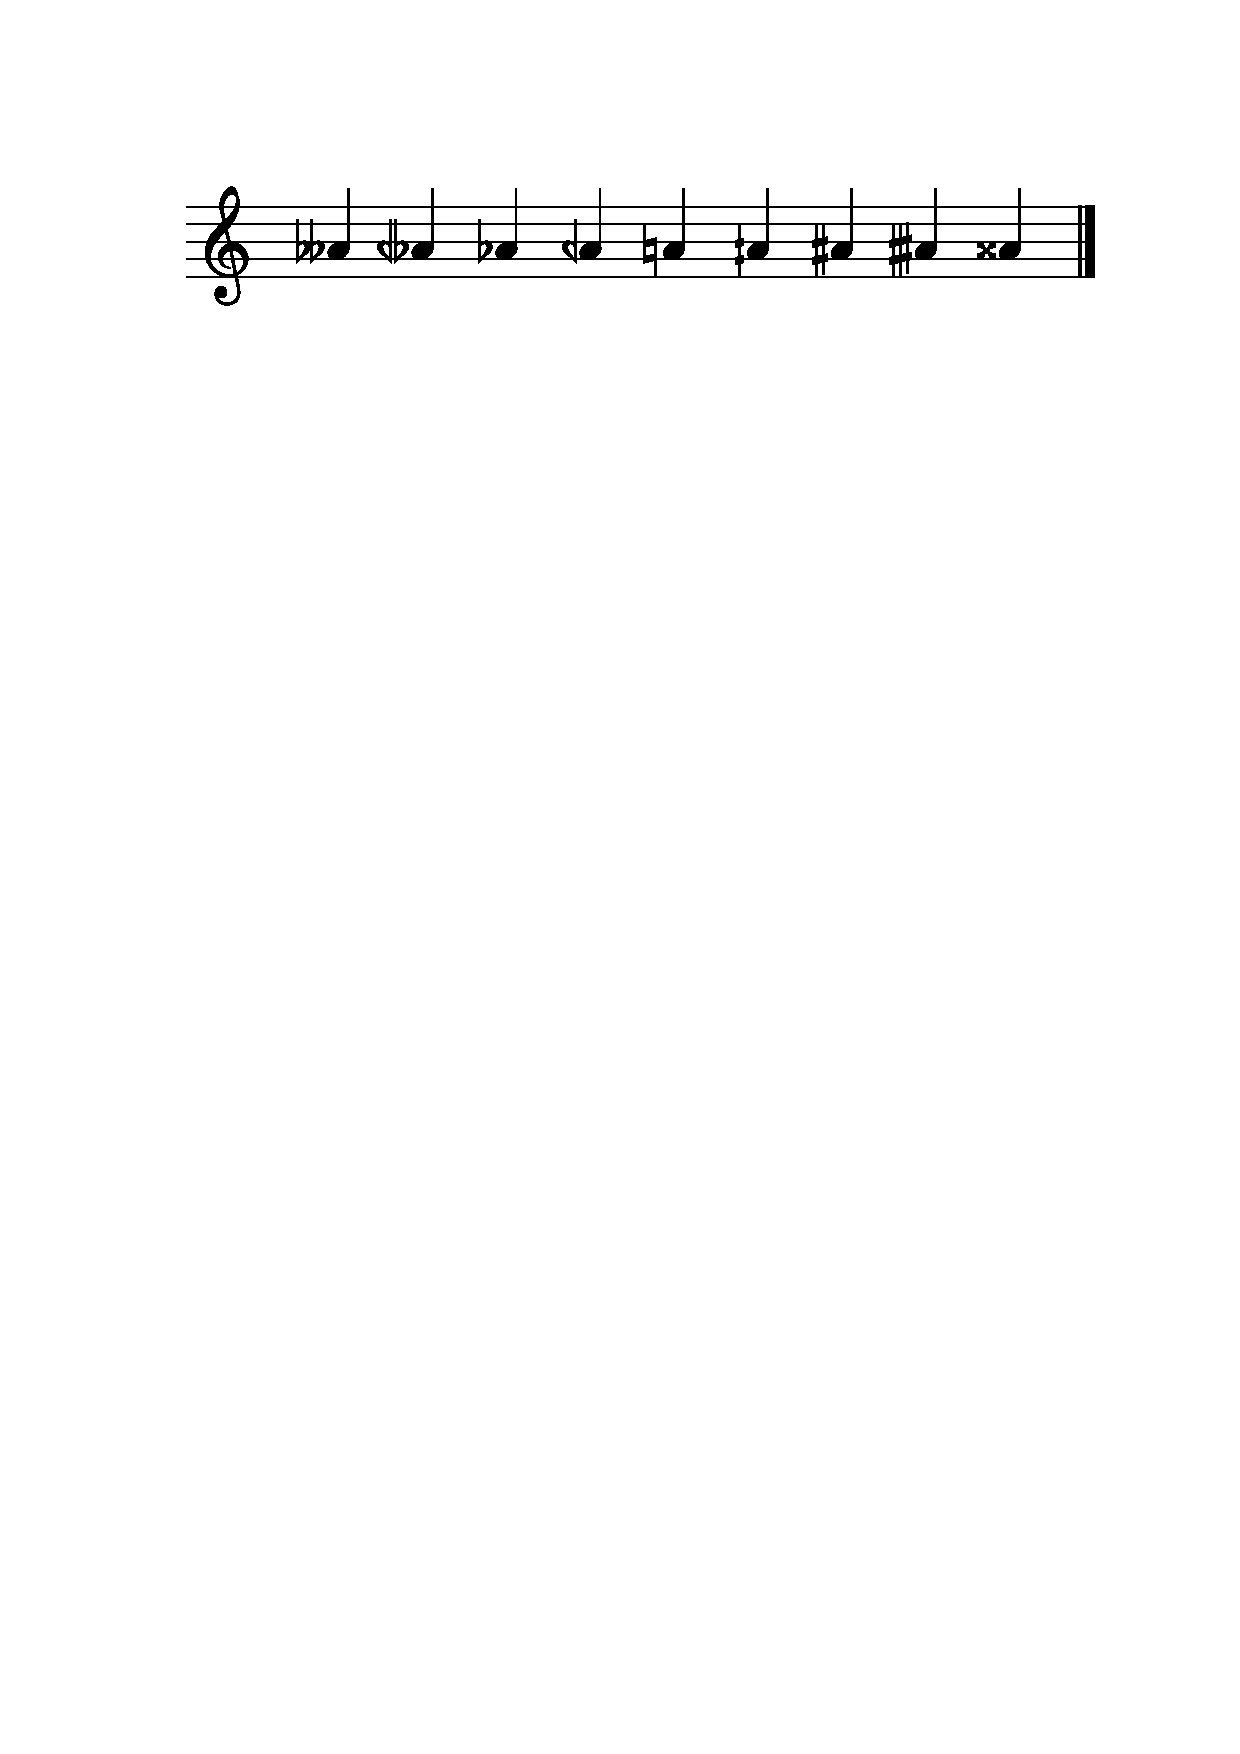
\includegraphics[width=\columnwidth]{img/partitions/alter.pdf}
\caption{Microtonalité}
\label{fig:alter}
\end{figure}

La microtonalité est également introduite dans les armures de clef libres. Elle s'exprime également sous forme de nombres flottants indiqués entre crochets.

\exemple
\begin{gmncode}
[
  \key<"free=c[1.5]g#b&a[-1.5]"> a g# 
  \alter<0.5> g  a \alter<1.5> g 
]
\end{gmncode}
Le résultat est présenté en figure \ref{fig:freekey}.
\begin{figure}[h]
\centering
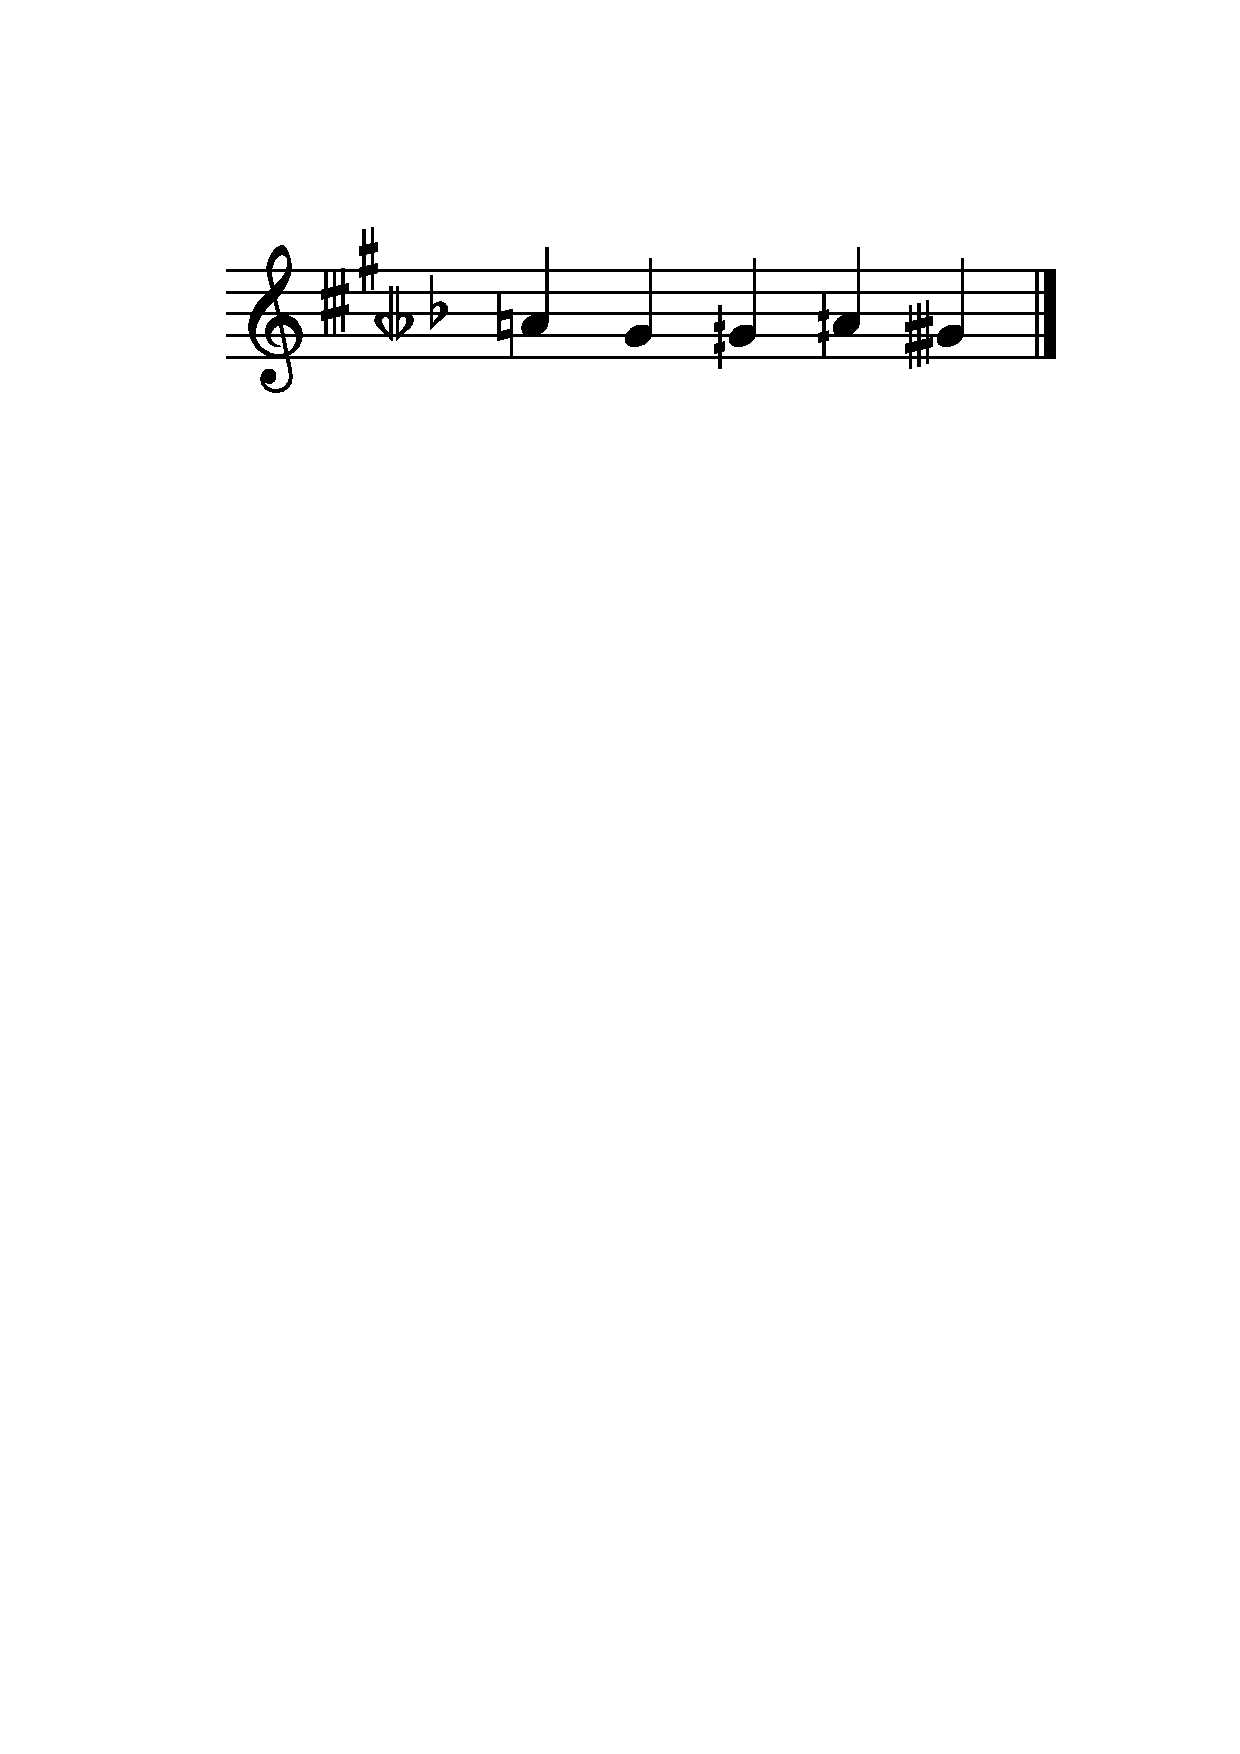
\includegraphics[width=0.75\columnwidth]{img/partitions/freekey.pdf}
\caption{Armure de clef libre avec microtonalité}
\label{fig:freekey}
\end{figure}


%**********************TETES DE NOTES *****************************
\subsection{Têtes de notes}\label{subsec:tetes_notes}
%
Nous avons choisi de rajouter à la librairie \guido\ 6 nouveaux symboles de têtes de note, afin de proposer un choix plus vaste à l'utilisateur. Dans l'ordre de la première portée de la figure \ref{fig:noteheads}, nous avons les nouveaux éléments suivants :
%
\begin{itemize}
    \item \emph{x} (une croix)
    \item \emph{diamond} (un diamant)
    \item \emph{round} (un rond)
    \item \emph{square} (un carré)
    \item \emph{triangle} (un triangle, pointe en haut)
    \item \emph{reversedTriangle} (un triangle, pointe en bas)
\end{itemize} 
\bigskip
%
\begin{figure}[h]
\centering
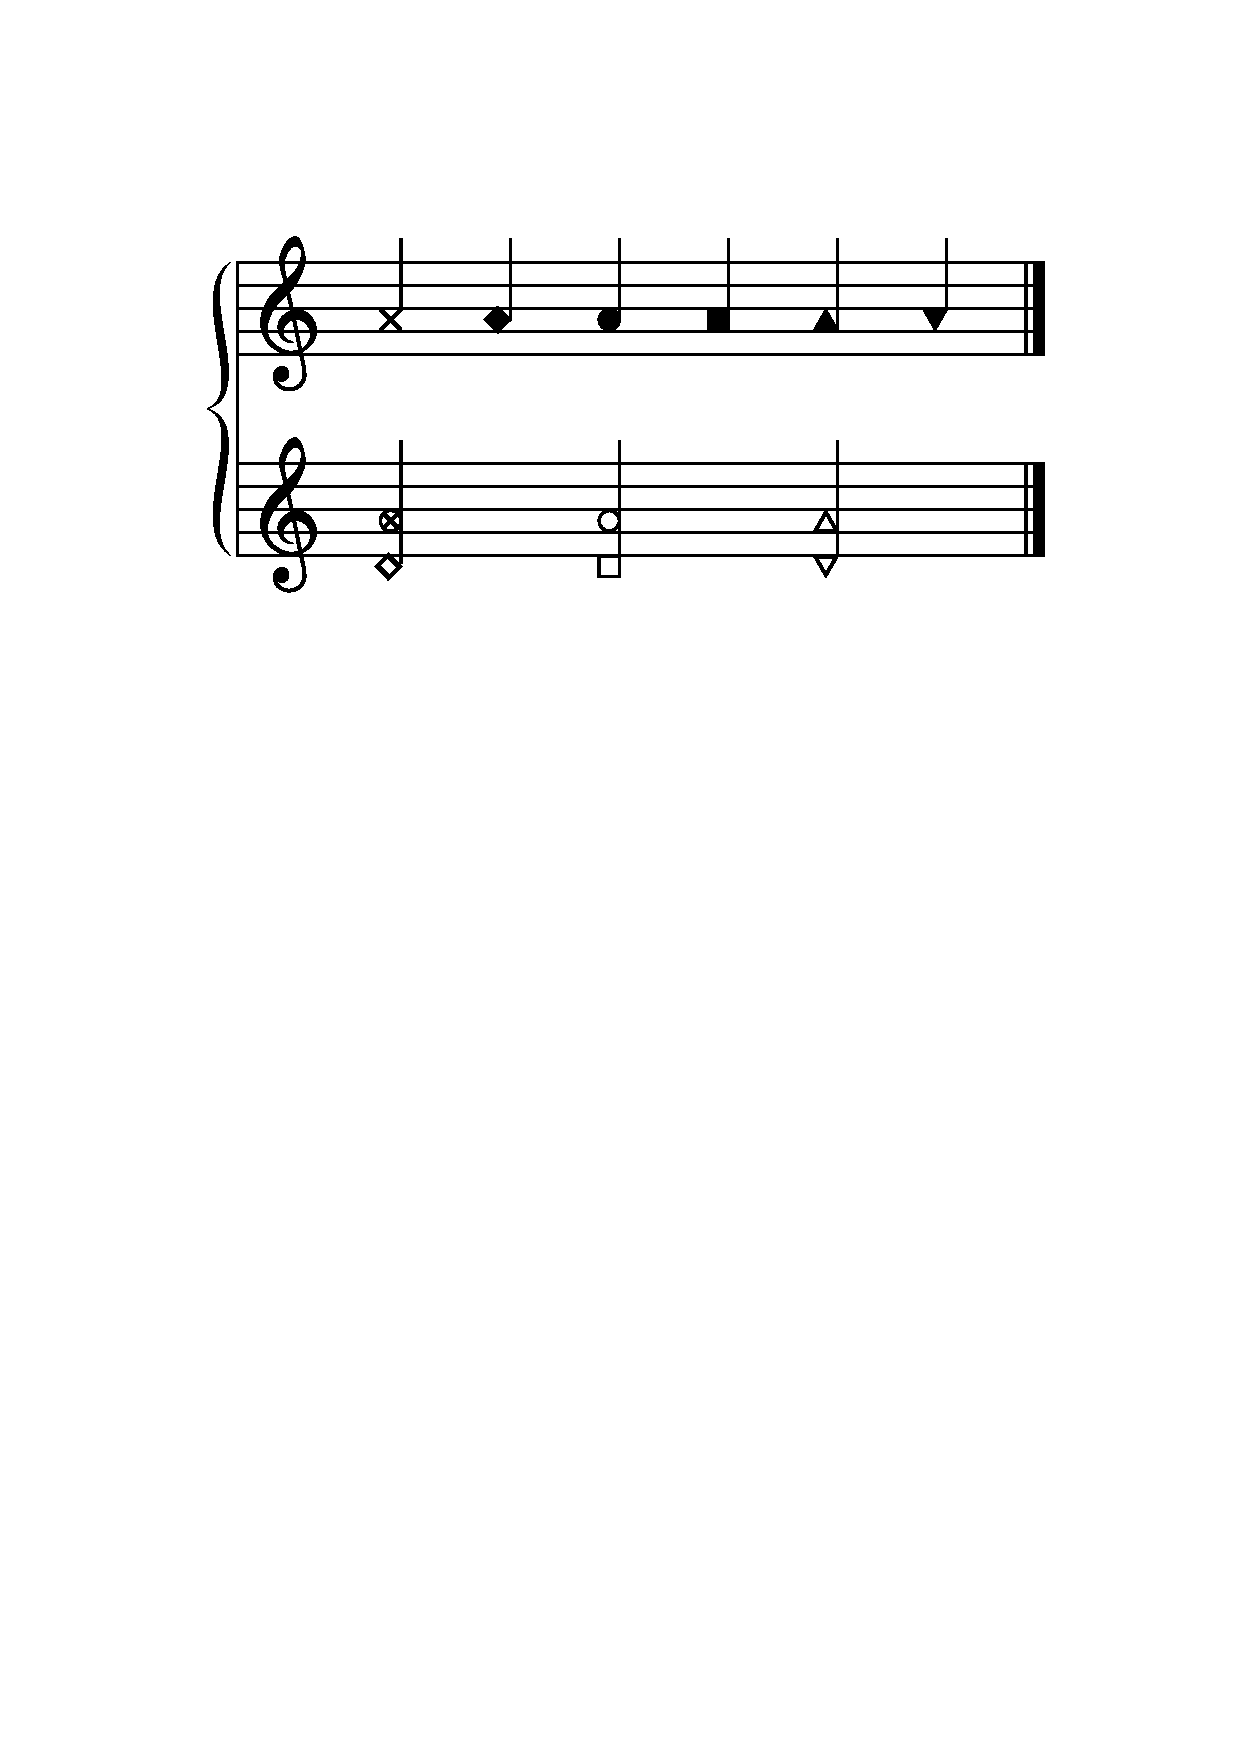
\includegraphics[width=6cm]{img/partitions/noteheads.pdf}
\caption{Les 6 nouveaux \emph{noteheads} ajoutés}
\label{fig:noteheads}
\end{figure}
%
Pour l'apparence graphique de ces éléments, nous nous sommes principalement inspirés de deux ouvrages, \emph{Behind Bars : The Definitive Guide to Music Notation} [4] et \emph{Music Notation in the Twentieth Century : A Practical Guidobook} [16].
%
Nous avons implémenté ces nouveaux éléments graphiques à l'aide du \emph{tag} \emph{noteFormat}, déjà existant. Celui-ci permet de modifier l'apparence des notes lui étant postérieures (couleur, taille, offset, etc.). Nous avons donc rajouté un attribut, \emph{style}, permettant à l'utilisateur de choisir l'apparence du \emph{notehead} des notes postérieures :

\begin{gmncode}
\noteFormat<style=noteHeadStyle> notes
\end{gmncode}

La première portée de l'exemple de la figure \ref{fig:noteheads} peut donc être générée avec le code \textsc{Guido} suivant:

\begin{gmncode}
[
  \noteFormat<style="x"> a
  \noteFormat<style="diamond"> a
  \noteFormat<style="round"> a
  \noteFormat<style="square"> a
  \noteFormat<style="triangle"> a
  \noteFormat<style="reversedTriangle"> a
]
\end{gmncode}
\bigskip

Ce travail d'implémentation a été décomposé en plusieurs étapes:
\begin{itemize}
    \item dessin vectoriel des nouveaux \emph{noteheads} (selon les ouvrages référents);
    \item implémentation du nouvel attribut du \emph{tag} \emph{noteFormat};
    \item derniers ajustements nécessaires pour un bon rendu visuel.
\end{itemize}

Quelques ajustements graphiques assez précis ont dû être réalisés pour parfaire le travail:
\begin{itemize}
    \item insertion d'un offset horizontal variable selon le symbole choisi, l'orientation de la hampe, l'utilisation en accord ou non (les accords pouvant posséder des \emph{noteheads} différents pour chacune de leurs notes);
    \item adaptation de la longueur de la hampe selon le type symbole utilisé (par exemple, différence de longueur entre le \emph{triangle} et le \emph{reversedTriangle}).
\end{itemize}


%**************************** COMPLEX METER ********************************
\subsection{Métriques complexes}\label{subsec:metriques}

% Pourquoi le texte n'est pas justifié ?
La possibilité d'insérer une métrique complexe a été introduite avec la version 1.52 de la librairie \guido. Elle offre à l'utilisateur la possibilité d'utiliser, graphiquement, une somme en place et lieu de la métrique habituelle, composée d'un seul nombre. Sa syntaxe est exactement la même que pour une métrique normale, il suffit de remplacer le numérateur par une somme, comme le montre l'exemple ci-dessous.

\exemple\\
Le code suivant produit le résultat présenté en figure \ref{fig:complexMeter}.
\begin{gmncode}
[
  \meter<"3+3+2/4"> a b g
]
\end{gmncode}

\begin{figure}[h]
\centering
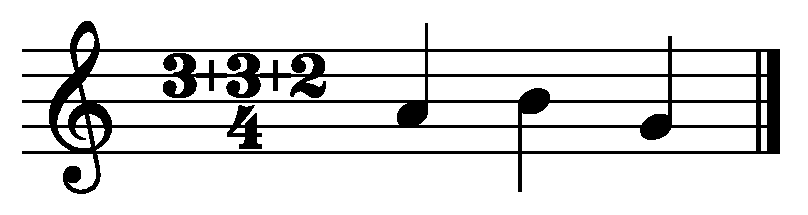
\includegraphics[width=50mm]{img/partitions/complexMeter.pdf}
\caption{Métrique complexe}
\label{fig:complexMeter}
\end{figure}

%**************************** CLUSTERS ********************************
\subsection{Clusters}\label{subsec:clusters}

Un \emph{cluster} est un accord musical contenant plusieurs notes consécutives. Il peut par exemple être effectué sur un piano, où il se joue en déclenchant des touches contiguës (en utilisant son avant-bras, par exemple).

Il a été décidé de spécifier les \emph{clusters} par un \emph{range-tag} s'appliquant à des accords de deux notes: les notes extrêmes du \emph{cluster} (les autres notes éventuelles seront ignorées) :

\begin{gmncode}
\cluster<param-list>(chord-series)
\end{gmncode}


%
\begin{figure}[h]
\centering
\begin{gmncode}
[
  \cluster({a, d} {c/8, f}
    {a/2, d2} {f/1, c1})
]
\end{gmncode}
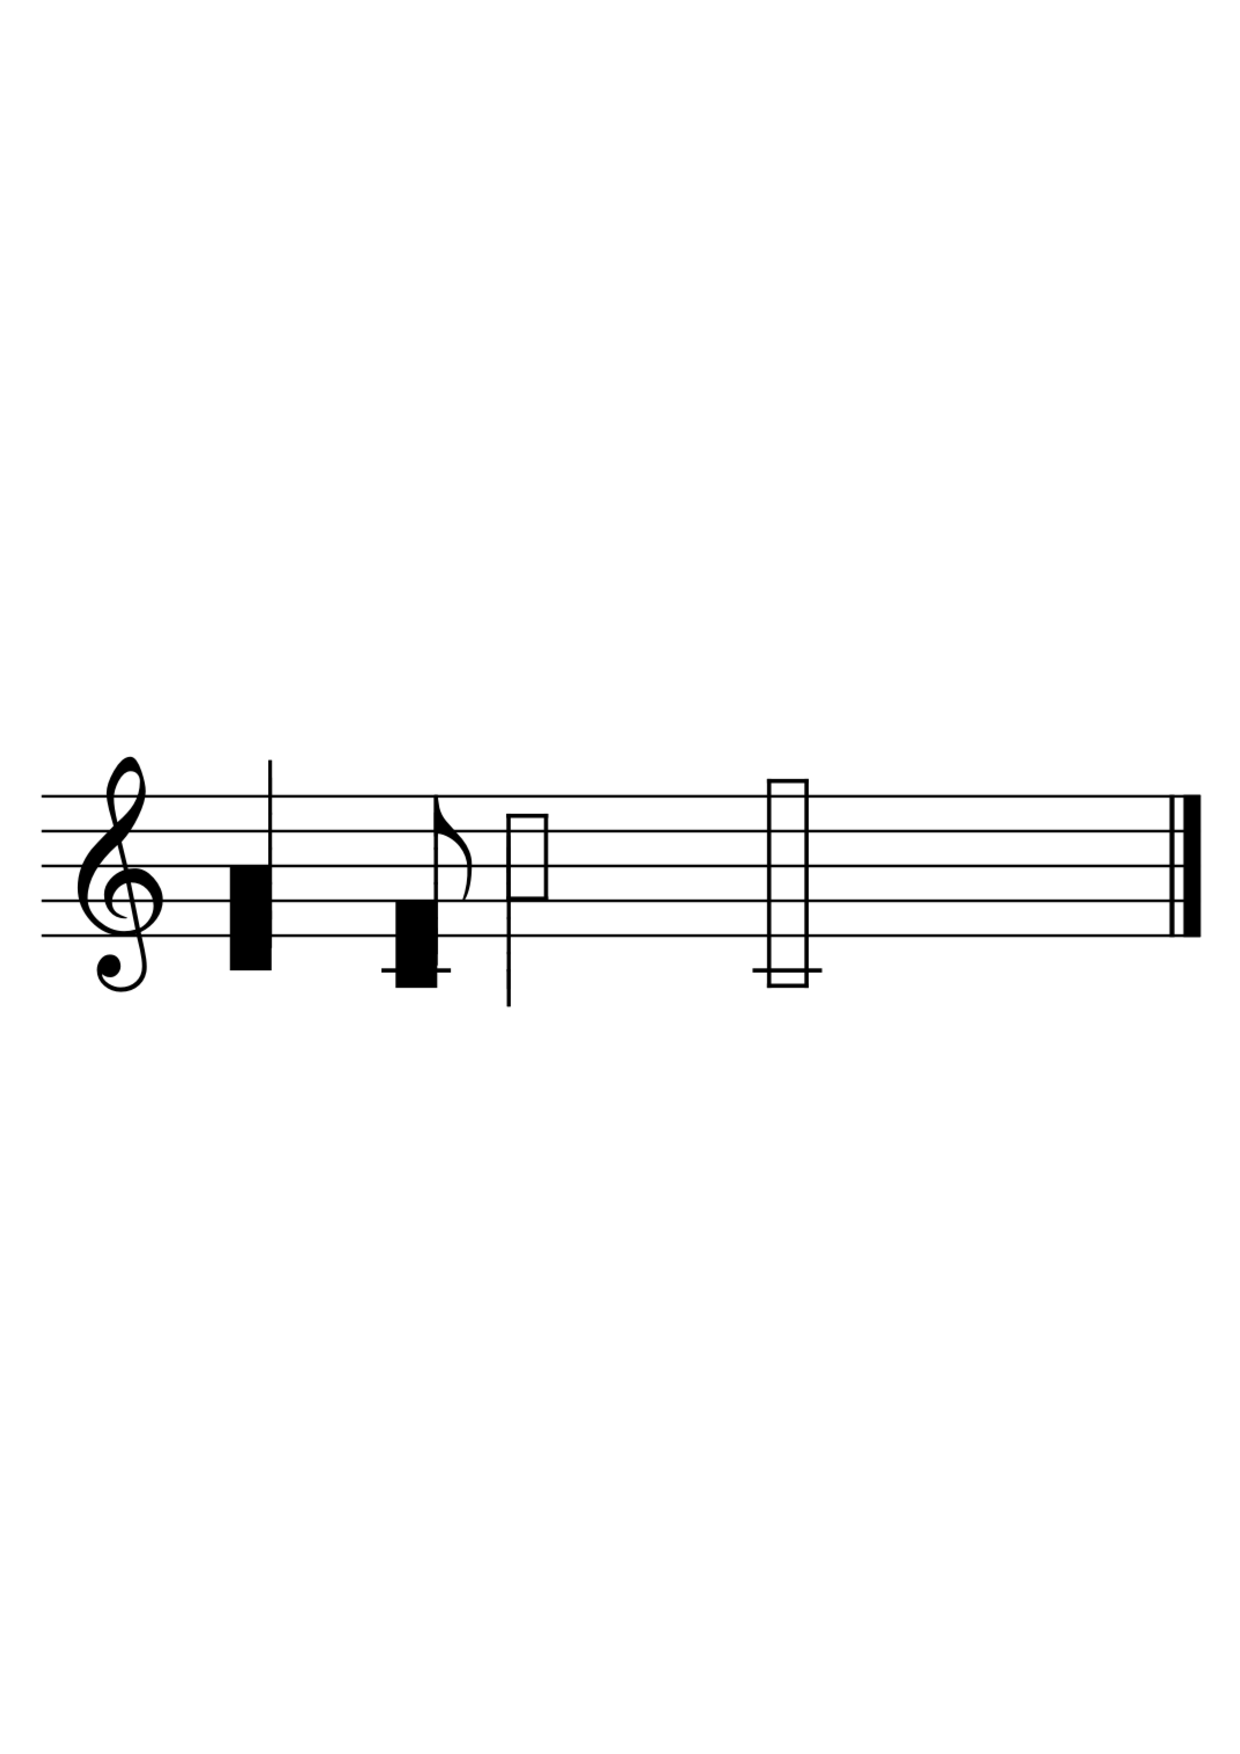
\includegraphics[width=50mm]{img/partitions/cluster.pdf}
\caption{\emph{Cluster}}
\label{fig:cluster}
\end{figure}
%

Comme l'indique en partie la figure \ref{fig:cluster}, les choix, faits à partir d'ouvrages référents, ont été les suivants:
\begin{itemize}
	\item le \emph{cluster} est représenté par un rectangle;
	\item ce rectangle est plein ou vide, selon la durée du \emph{cluster};
	\item la hampe est conservée pour garder l'indication de la durée.
\end{itemize}

Nous avons également fait en sorte que l'utilisateur puisse personnaliser au maximum le nouvel élément de la librairie \guido. En plus des habituels \emph{size}, \emph{dx}, \emph{dy} et \emph{color}, les attributs \emph{hdx} et \emph{hdy} ont été implémentés afin de pouvoir introduire un décalage s'appliquant au \emph{notehead} seulement. Au niveau de l'interaction avec d'autres éléments et \emph{tags}, nous avons fait en sorte que noteFormat agisse également sur le \emph{cluster}. D'autre part, la gestion du forçage de l'orientation des \emph{noteheads} a de même été prise en compte (\emph{tags} \emph{headsReverse}, \emph{headsLeft} et \emph{headsRight}) (cf. figure \ref{fig:clusterInteractions}).

%
\begin{figure}[h]
\centering
\begin{gmncode}
[
  \cluster<color="red", hdx=1, hdy=3>({a})
  \cluster<size=0.5>({f,c2})
  \noteFormat<color="purple">
  \headsReverse
  \cluster<color="green", size=2>({f, g2})
  \cluster<"blue">({d1/2, g})
]
\end{gmncode}
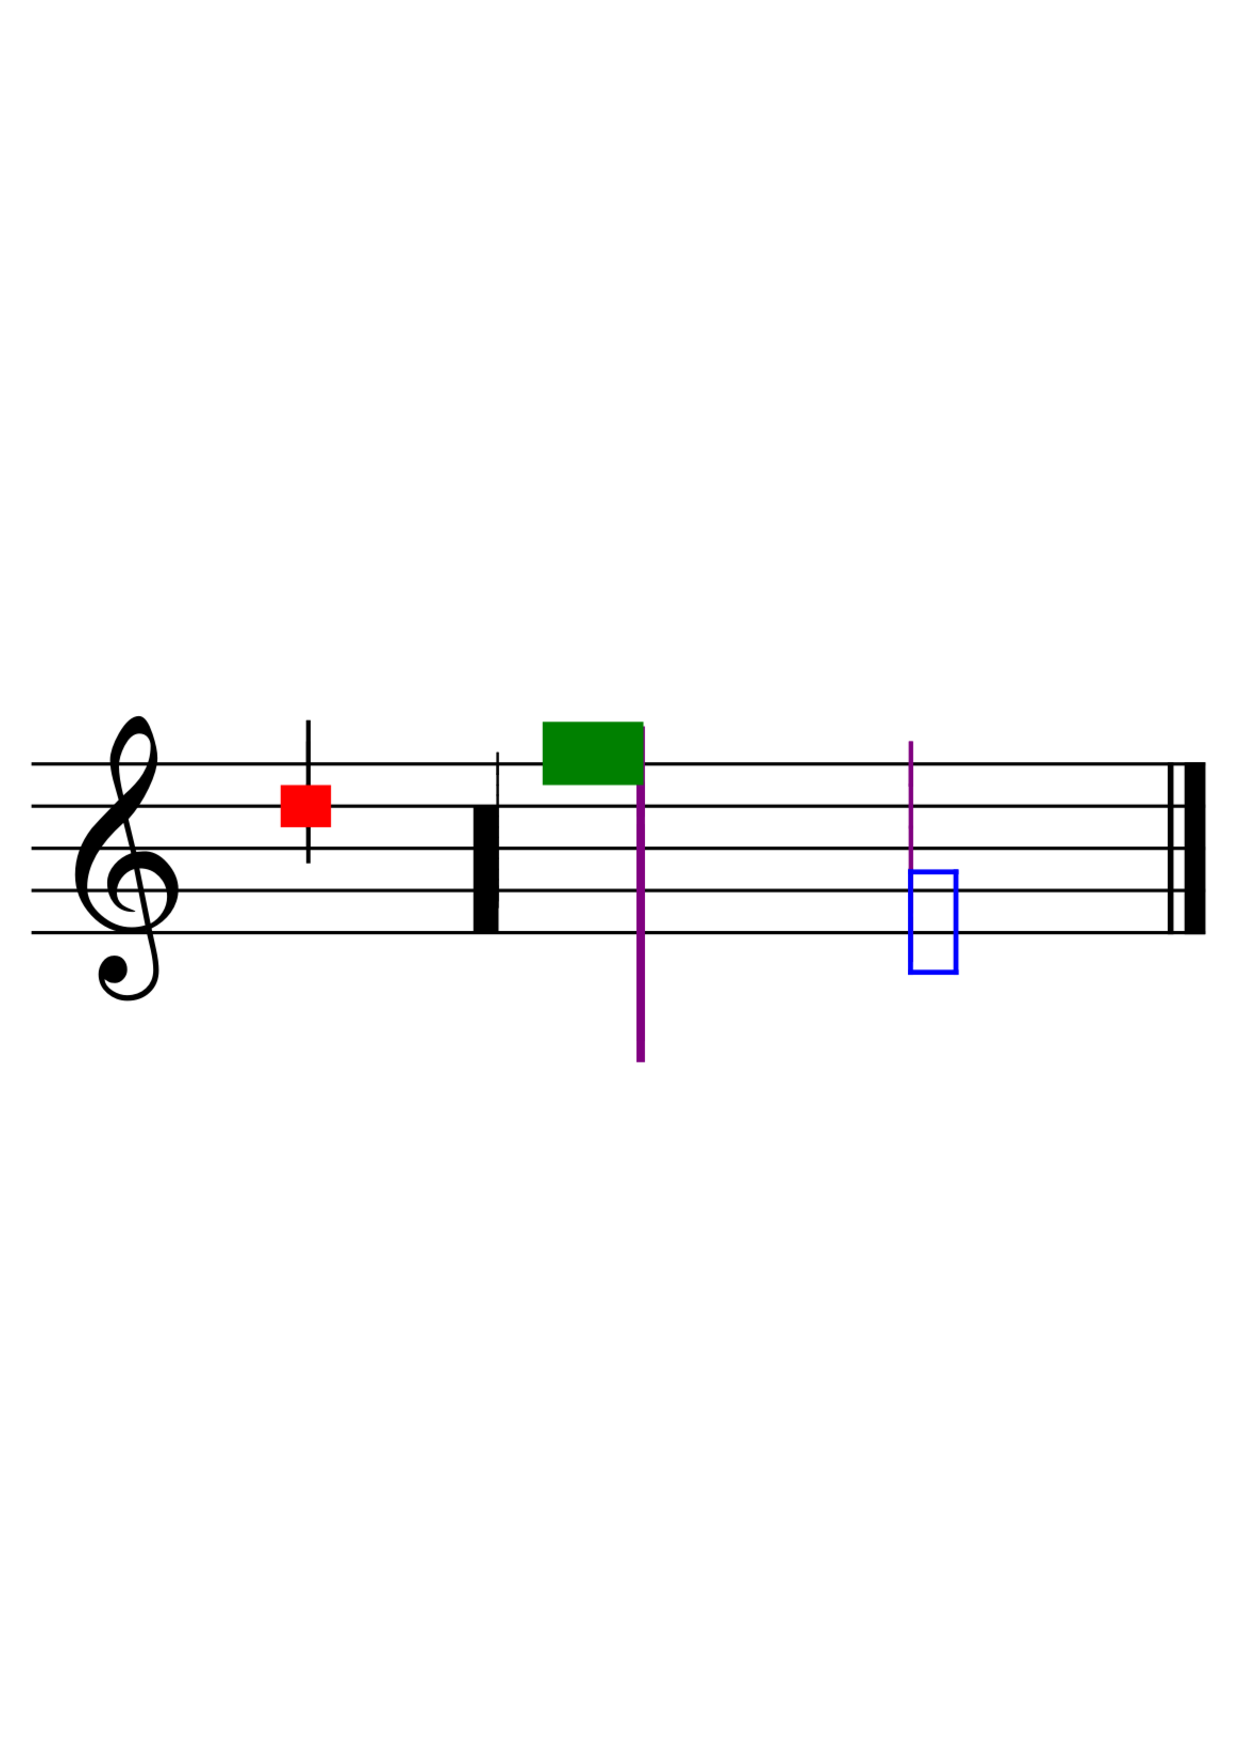
\includegraphics[width=45mm]{img/partitions/clusterInteractions.pdf}
\caption{Les interactions avec d'autres \emph{tags}}
\label{fig:clusterInteractions}
\end{figure}
%


%***************GLISSANDO************************
\subsection{Glissandi}\label{subsec:glissando}

Le \emph{glissando} se présente classiquement comme une ligne joignant deux notes décalées dans le temps ( Figure \ref{fig:glissandoSimple} ), indiquant ainsi un glissement, continu ou non suivant le type d'instrument, d'une hauteur à l'autre.

Dans un souci d'efficacité, il fallait pouvoir décrire un \emph{glissando} seul ou plusieurs \emph{glissandi} à la suite de la manière la plus simple et intuitive possible. 

\begin{gmncode}
\glissando<params>( notes )
\end{gmncode}

Il paraissait important de donner la possibilité à l'utilisateur de n'écrire qu'une seule fois le \emph{tag} pour décrire plusieurs \emph{glissandi} consécutifs, contrairement à la description de lilypond où le \emph{tag} doit être répété entre chaque note. Ainsi le \emph{range-tag} (\emph{tag} possédant une durée) apparaissait comme la meilleure solution pour décrire un ou plusieurs \emph{glissandi} : toutes les notes comprises dans les parenthèses seraient prises en compte et liées les unes aux autres par des \emph{glissandi}. L'algorithme de démultiplication d'un même \emph{tag} et de répartition de celui-ci est fortement inspiré de celui du \emph{tie}, ou liaison de prolongation, qui doit également créer une liaison entre chacune des notes affectées.
\\

\begin{figure}[h]
\centering

\begin{gmncode}
[ \glissando( g b d ) ]
\end{gmncode}

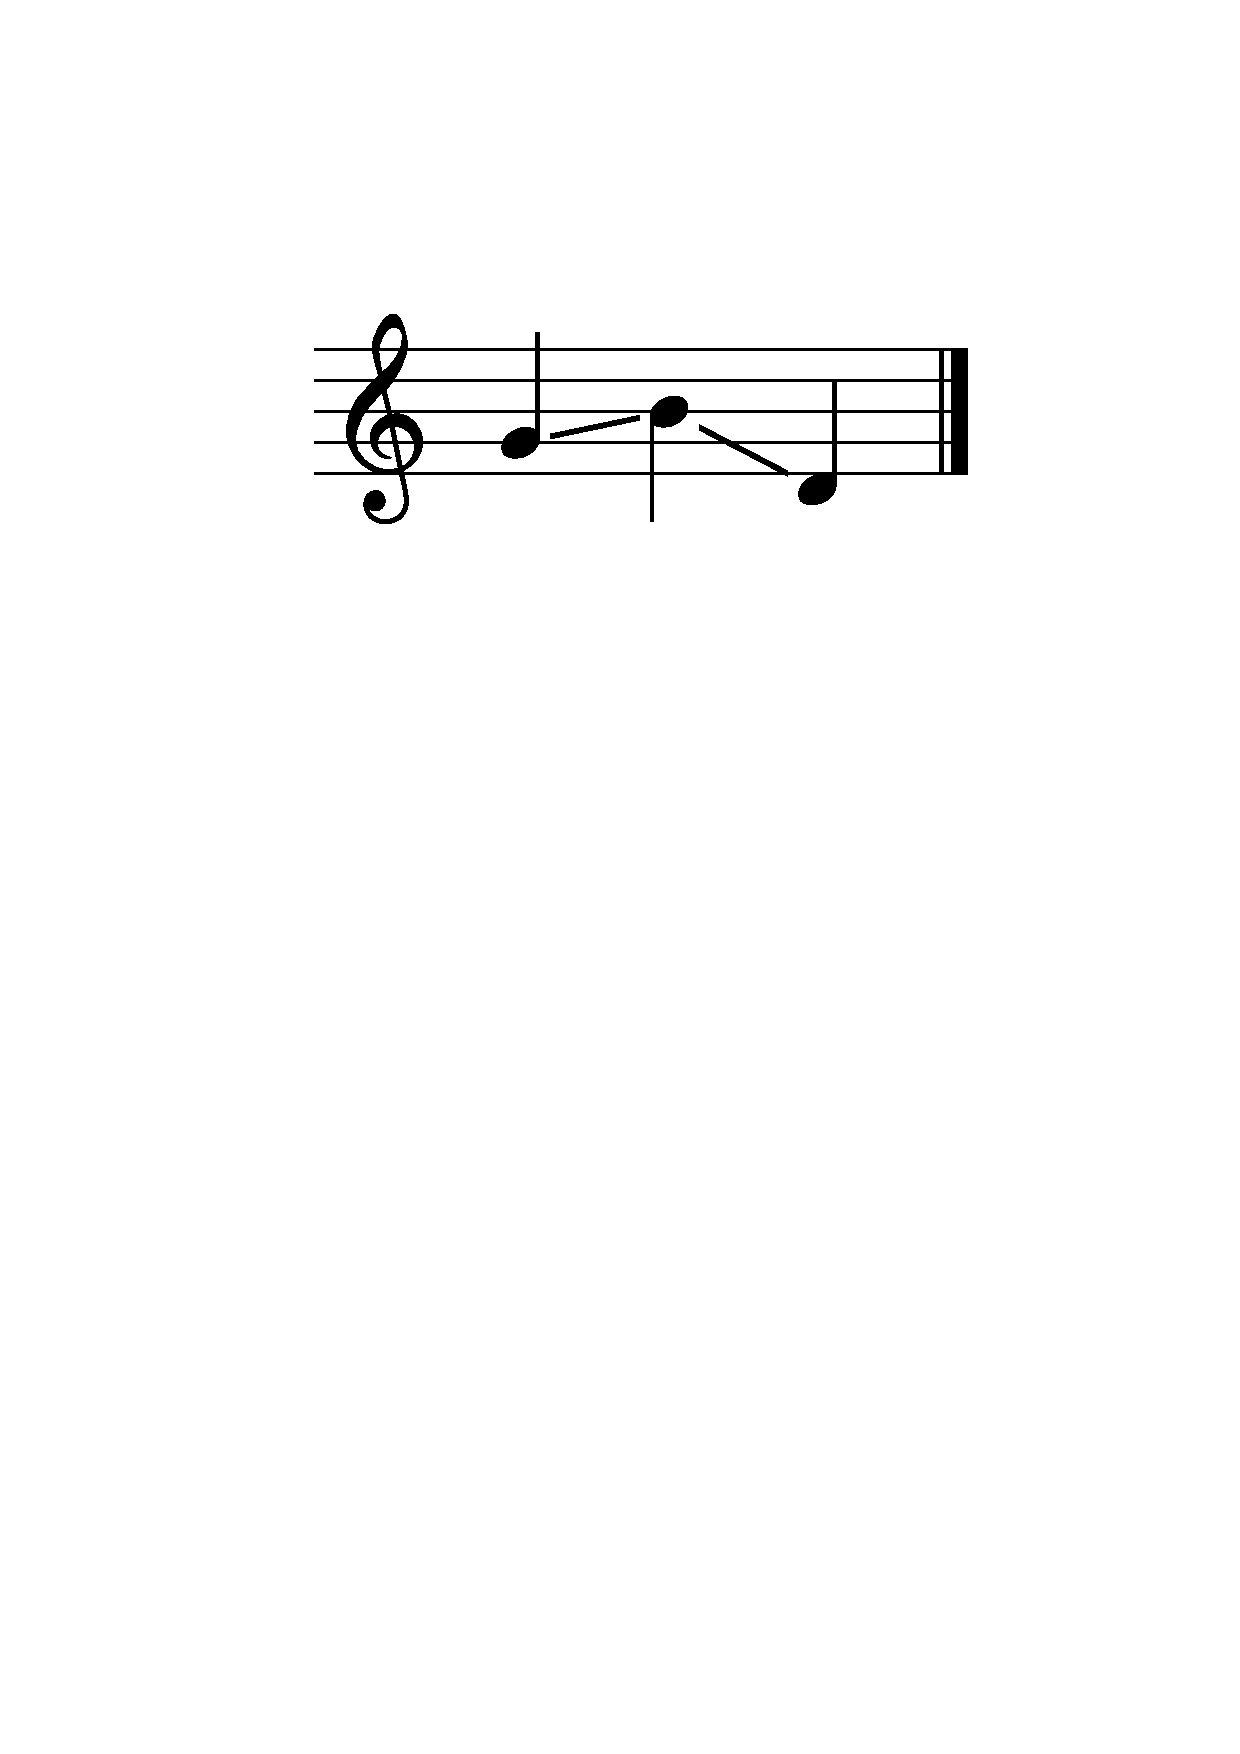
\includegraphics[width=35mm]{img/glissando1.pdf}
\caption{Glissando}
\label{fig:glissandoSimple}
\end{figure}




% *********************** FEATHERED BEAM ****************************
\subsection{Liens de croches en soufflet (feathered beaming)}\label{subsec:featheredBeaming}
\bigskip

\begin{gmncode}
\fBeam<params>( notes )
  params : 
    - durations="firstDur, lastDur" : 
      durée des première et dernière notes
    - drawDuration : 
      indication de la durée totale

\end{gmncode}

Décrite par Gardner Read \cite{read1969music} comme "a highly graphic representation of rythmic flexibility"(p.94), cette notation contemporaine d'un accelerando ou ritardando à travers les liens de croches est, de manière générale, encore peu répandue dans les ouvrages de théorie, et se résume souvent à des cas simples, partant ou arrivant à la simple croche, c'est à dire partant ou arrivant vers un unique point. Pourtant il paraît intéressant de pouvoir offrir la possiblité aux compositeurs de décrire le passage entre n'importe quelles valeurs : par exemple d'une double-croche à une triple-croche, ou d'une quadruple-croche à une double-croche... (Figure \ref{fig:fbeamcomplex})

\begin{figure}[h]
\centering
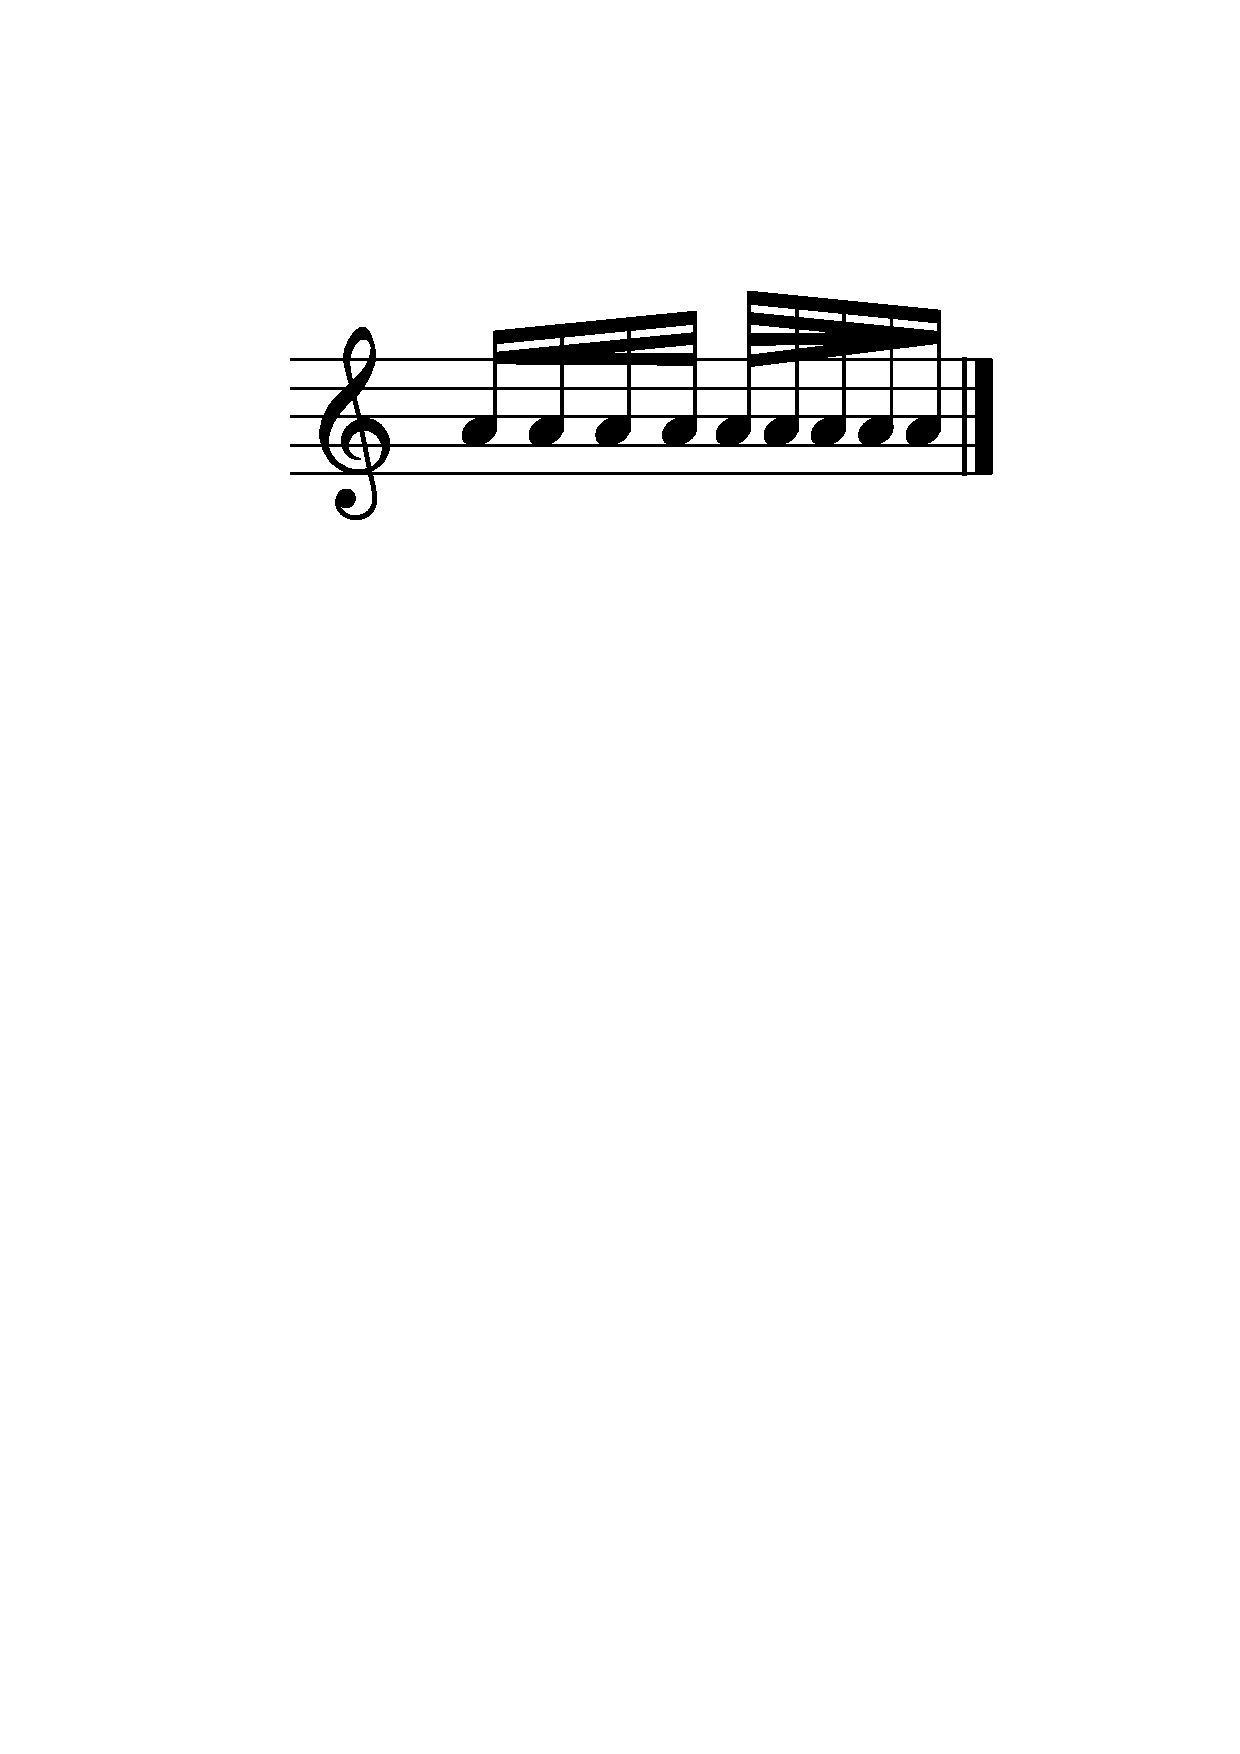
\includegraphics[width=40mm]{img/fbeamcomplex.pdf}
\caption{Exemple de \emph{feathered beams} plus complexes}
\label{fig:fbeamcomplex}
\end{figure}

Dans un désir de simplicité, il a été décidé de décrire par un seul \emph{range-tag} un seul groupe de notes liées, correspondant à un point de départ et un point d'arrivée uniques.

\begin{figure}[h]
\centering
\begin{gmncode}
[ 
  \fBeamBegin:1 
  c/8 d e/16 
  \fBeamBegin:2 f/32 \fBeamEnd:1 
  e/16 d/8 c
  \fBeamEnd:2 
]
\end{gmncode}
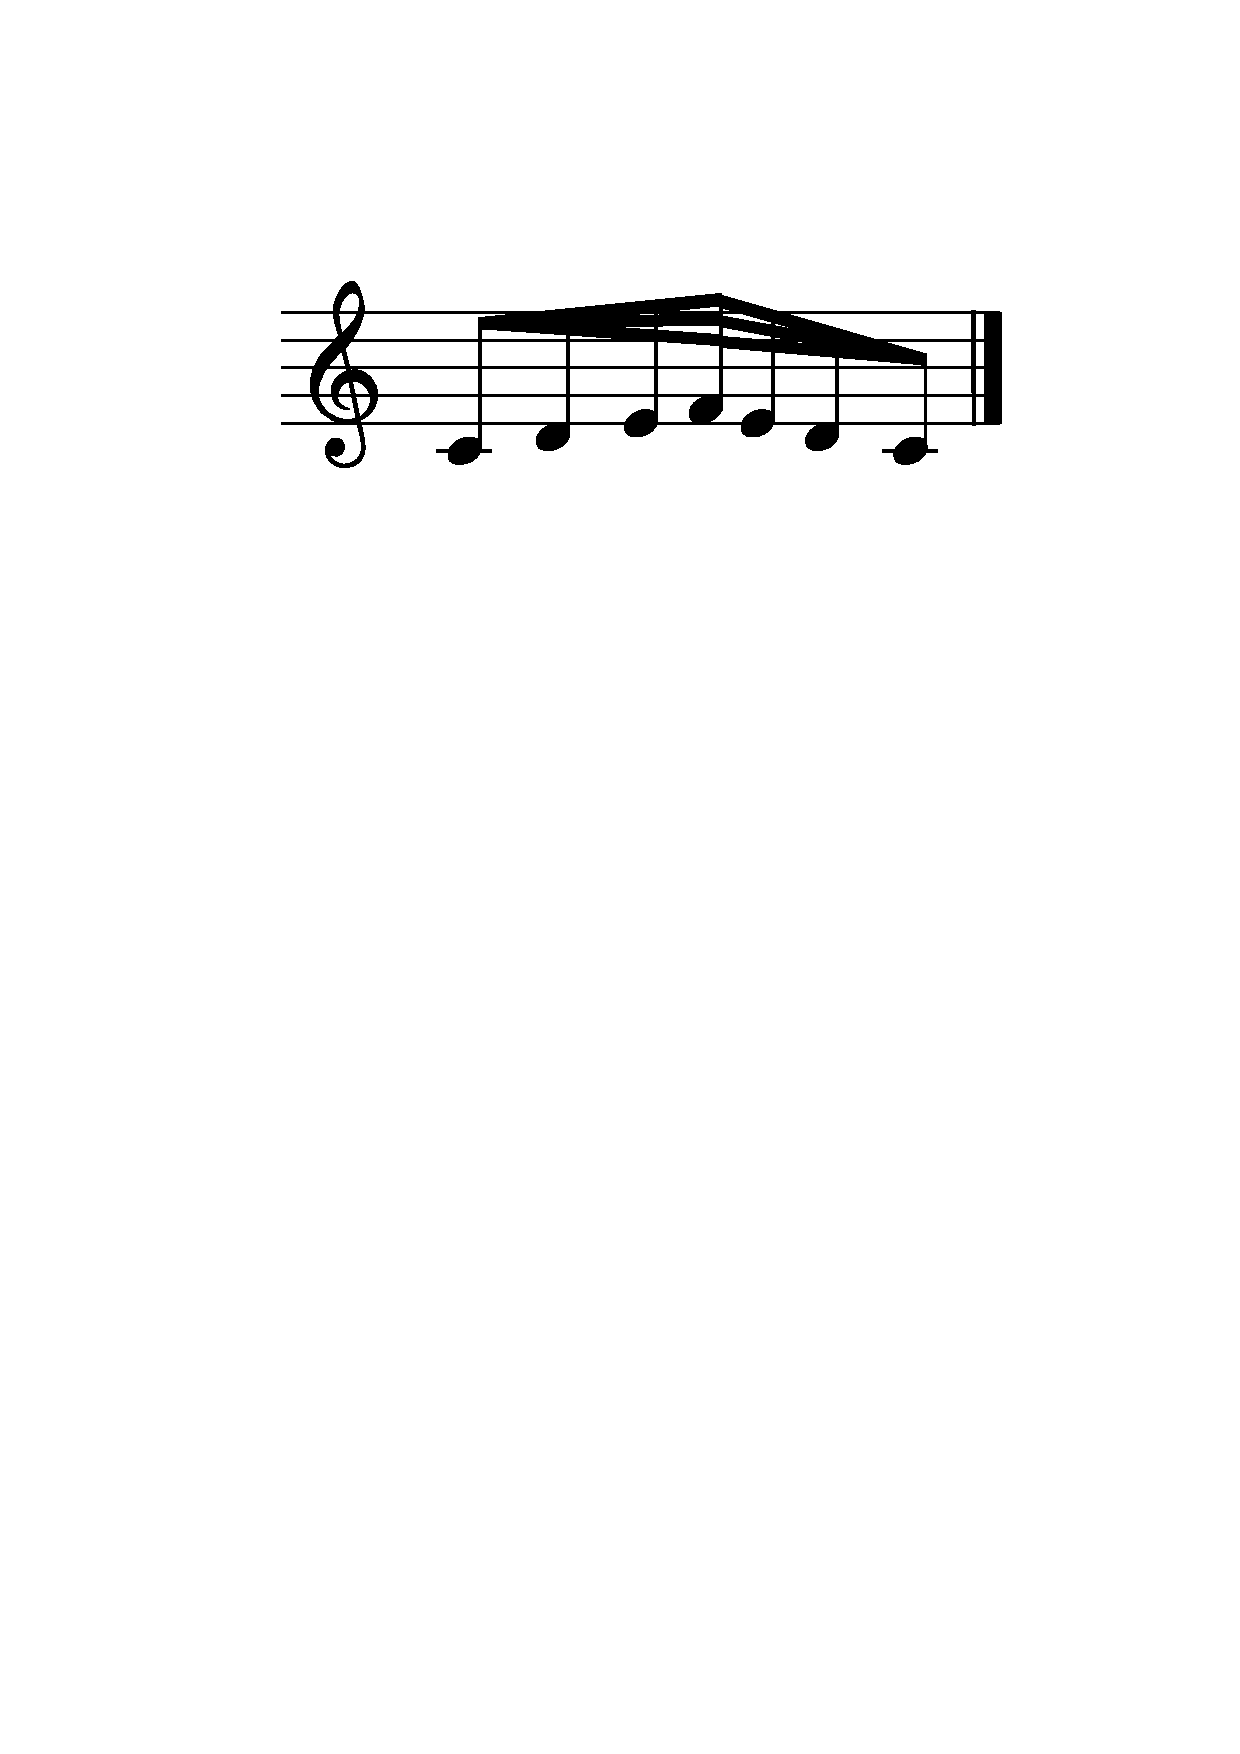
\includegraphics[width=45mm]{img/fBeamChaine.pdf}
\caption{\emph{Feathered beams} chaînés}
\label{fig:fbeamchain}
\end{figure}

Il est cependant possible de chaîner plusieurs \emph{feathered beams} grâce à la faculté du \emph{tag} à se séparer en \emph{\textbackslash{}fBeamBegin} et \emph{\textbackslash{}fBeamEnd}, permettant alors, non seulement de chaîner deux \emph{beams} par une note (Figure \ref{fig:fbeamchain}), mais aussi de les faire se chevaucher sur plusieurs notes.
\bigskip

% question de voix simultanées
% lilypond : 
% \override Beam #'grow-direction = #LEFT
% \featherDurations #(ly:make-moment 2 1)
% { c16[ c c c c c c c] }

On remarque que, même dans un ouvrage tel que celui d'Elaine Gould \cite{gould2011behind}, peu de détails sont donnés sur cette notation, et on se heurte rapidement à des incohérences telles que celle de la figure \ref{fig:incoherence} tirée de "Behind Bars" : on veut faire tenir en un temps une croche et quatre notes de durées inférieures à la croche mais supérieures à la triple-croche. 

\begin{figure}[h]
\centering
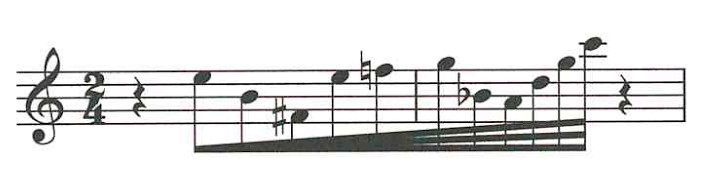
\includegraphics[width=8cm]{img/behindbars.jpg}
\caption{Exemple d'incohérence entre la durée totale et les durées individuelles des notes d'un groupe lié. (Behind Bars, p.158) }
\label{fig:incoherence}
\end{figure}

Ce manque d'une exacte cohérence entre tempo et aspect graphique est également souligné par Kurt Stone \cite{stone1980music} : "Besides, the gradual increase or decrease in the number of beams makes exact indications of beat-units impossible" (p.124).

Ainsi on voit l'importance des choix de design de ce symbole, sur la manière de le décrire textuellement, de le dessiner en particulier dans le cas de plusieurs voix simultanés, et de manière générale sur la liberté laissée à l'utilisateur.
\\

Concernant les possibilités de description données à l'utilisateur. Nous avons vu que plusieurs critères pouvaient intervenir dans la description, et devaient pouvoir être imposés par l'utilisateur. Des paramètres qui peuvent être incohérents entre eux :
\begin{itemize}
\item le nombre de notes dans le groupe,
\item leurs durées individuelles et intrinsèques qui définissent également leur espacement,
\item la durée totale du groupe, dépendante directement des durées individuelles,
\item les durées de départ et d'arrivée qui définissent l'aspect graphique du \emph{feathered beam}.
\end{itemize}
\bigskip

Ces différents niveaux de description nous poussent à faire une claire distinction entre l'aspect temporel et l'aspect graphique de notre groupe de notes.  Il a été décidé de laisser au compositeur la liberté de donner à son \emph{feathered beam} l'aspect graphique qu'il désire, indépendamment des durées internes de ses notes. Il pourra ainsi jouer sur les espacements entre notes, sur le nombre de notes, et sur la durée totale de manière "classique" en imposant à chaque note une durée, et en veillant à ce que la somme de toutes les notes corresponde à la durée totale souhaitée. Cette durée totale peut être indiquée sur la partition grâce au paramètre \emph{drawDuration} (Figure \ref{fig:fbeamduree}).

\begin{figure}[h]
\centering
\begin{gmncode}
[ 
  \fBeam<drawDuration="true">
  ( a/8 a a/16 a a a/32 a ) 
]
\end{gmncode}
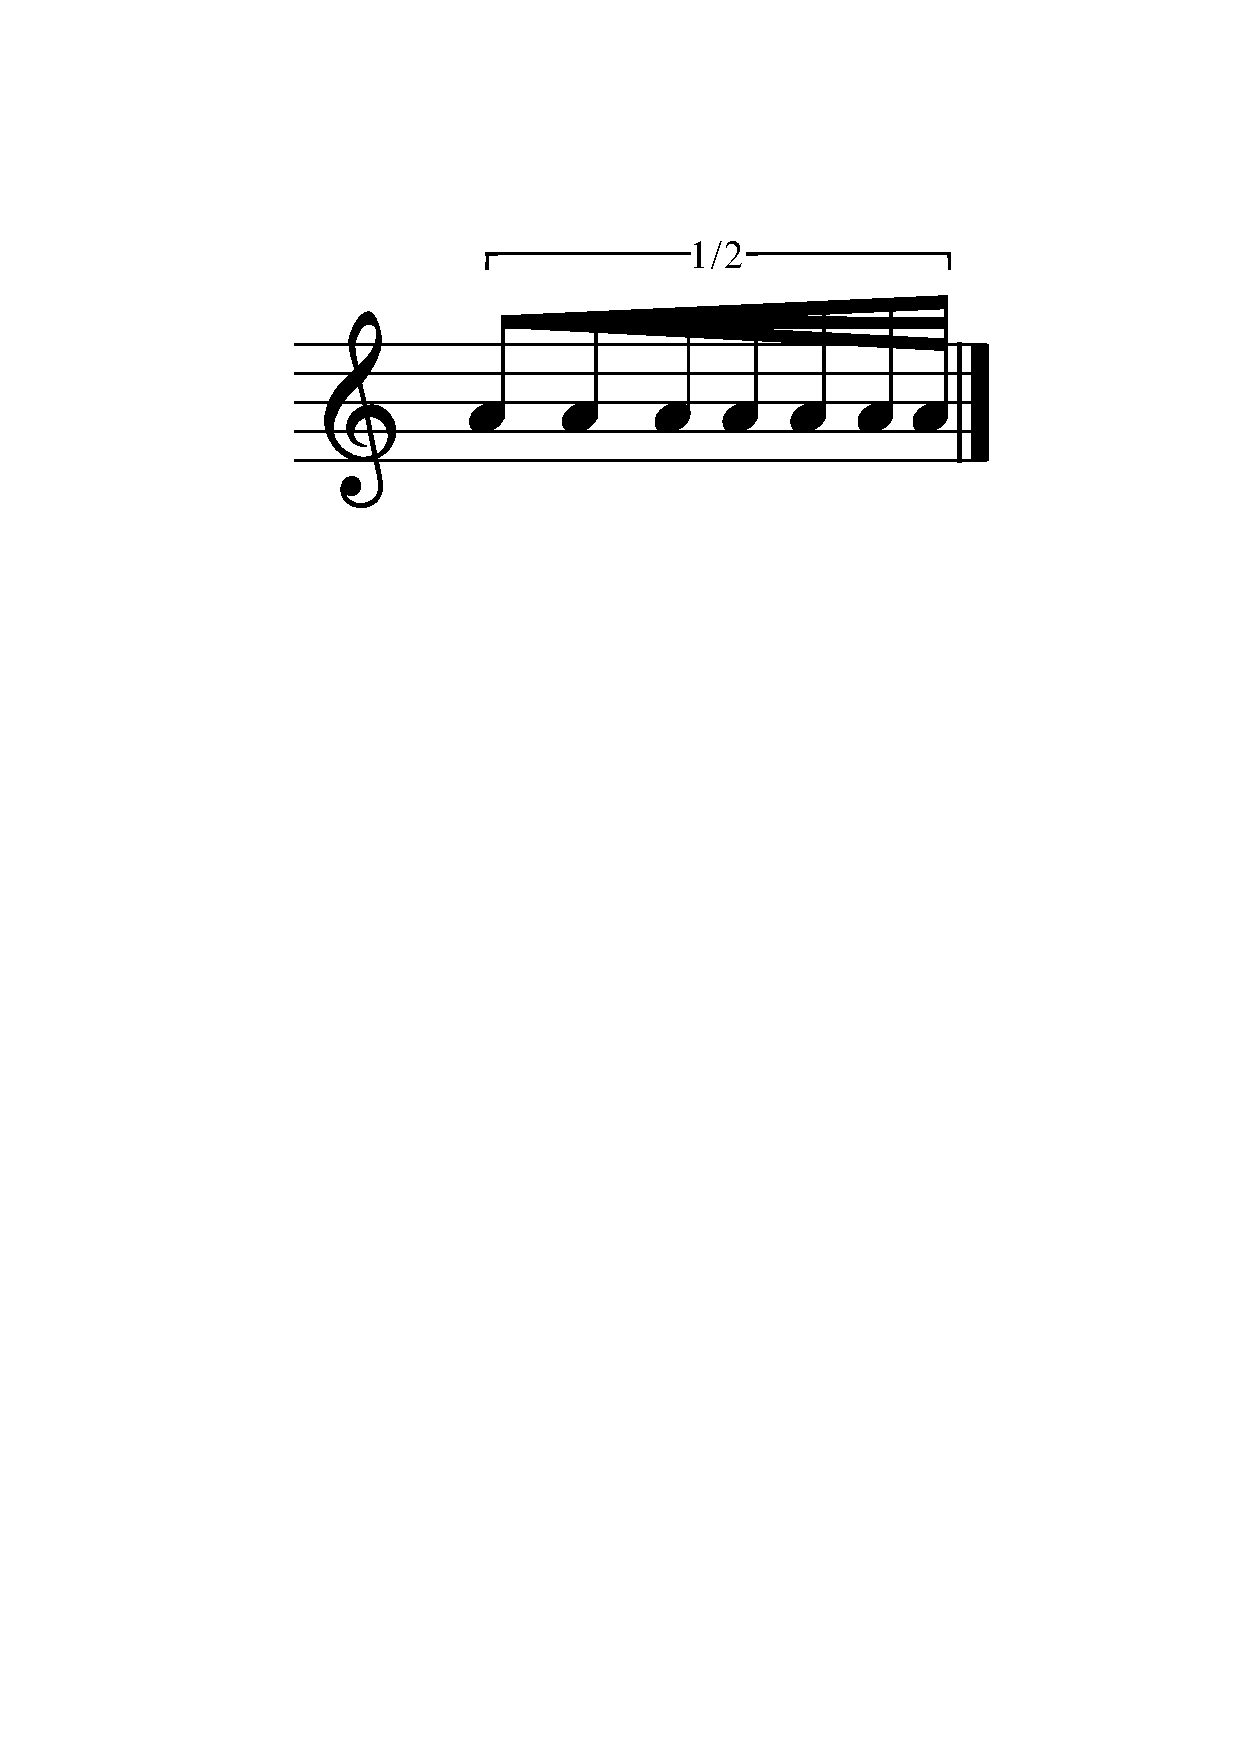
\includegraphics[width=40mm]{img/fbeamduree.pdf}
\caption{Représentation de la durée}
\label{fig:fbeamduree}
\end{figure}

Sans plus d'indication de sa part, l'aspect graphique suivra les durées réelles des notes et prendra comme points de départ et d'arrivée les durées des première et dernière notes.  C'est le cas de la Figure \ref{fig:fbeamduree}.

En revanche, le paramètre \emph{durations} pourra lui permettre d'imposer un aspect graphique tout autre, lui donnant ainsi la possibilité d'indiquer à l'interprète un changement de tempo plus ou moins important, et pas nécessairement cohérent avec les durées intrinsèques des notes, mais ayant du sens dans l'interprétation (Cf Figure \ref{fig:utilisateur}).

%%
\begin{comment}
Ainsi, les deux descriptions suivantes sont valides, mais pas équivalentes :
\\

\begin{figure}[h]
\centering
\begin{gmncode}
[ 
  \fBeam<drawDuration="true">
  (a/16 a a a/32 a/64 a) 
]
\end{gmncode}

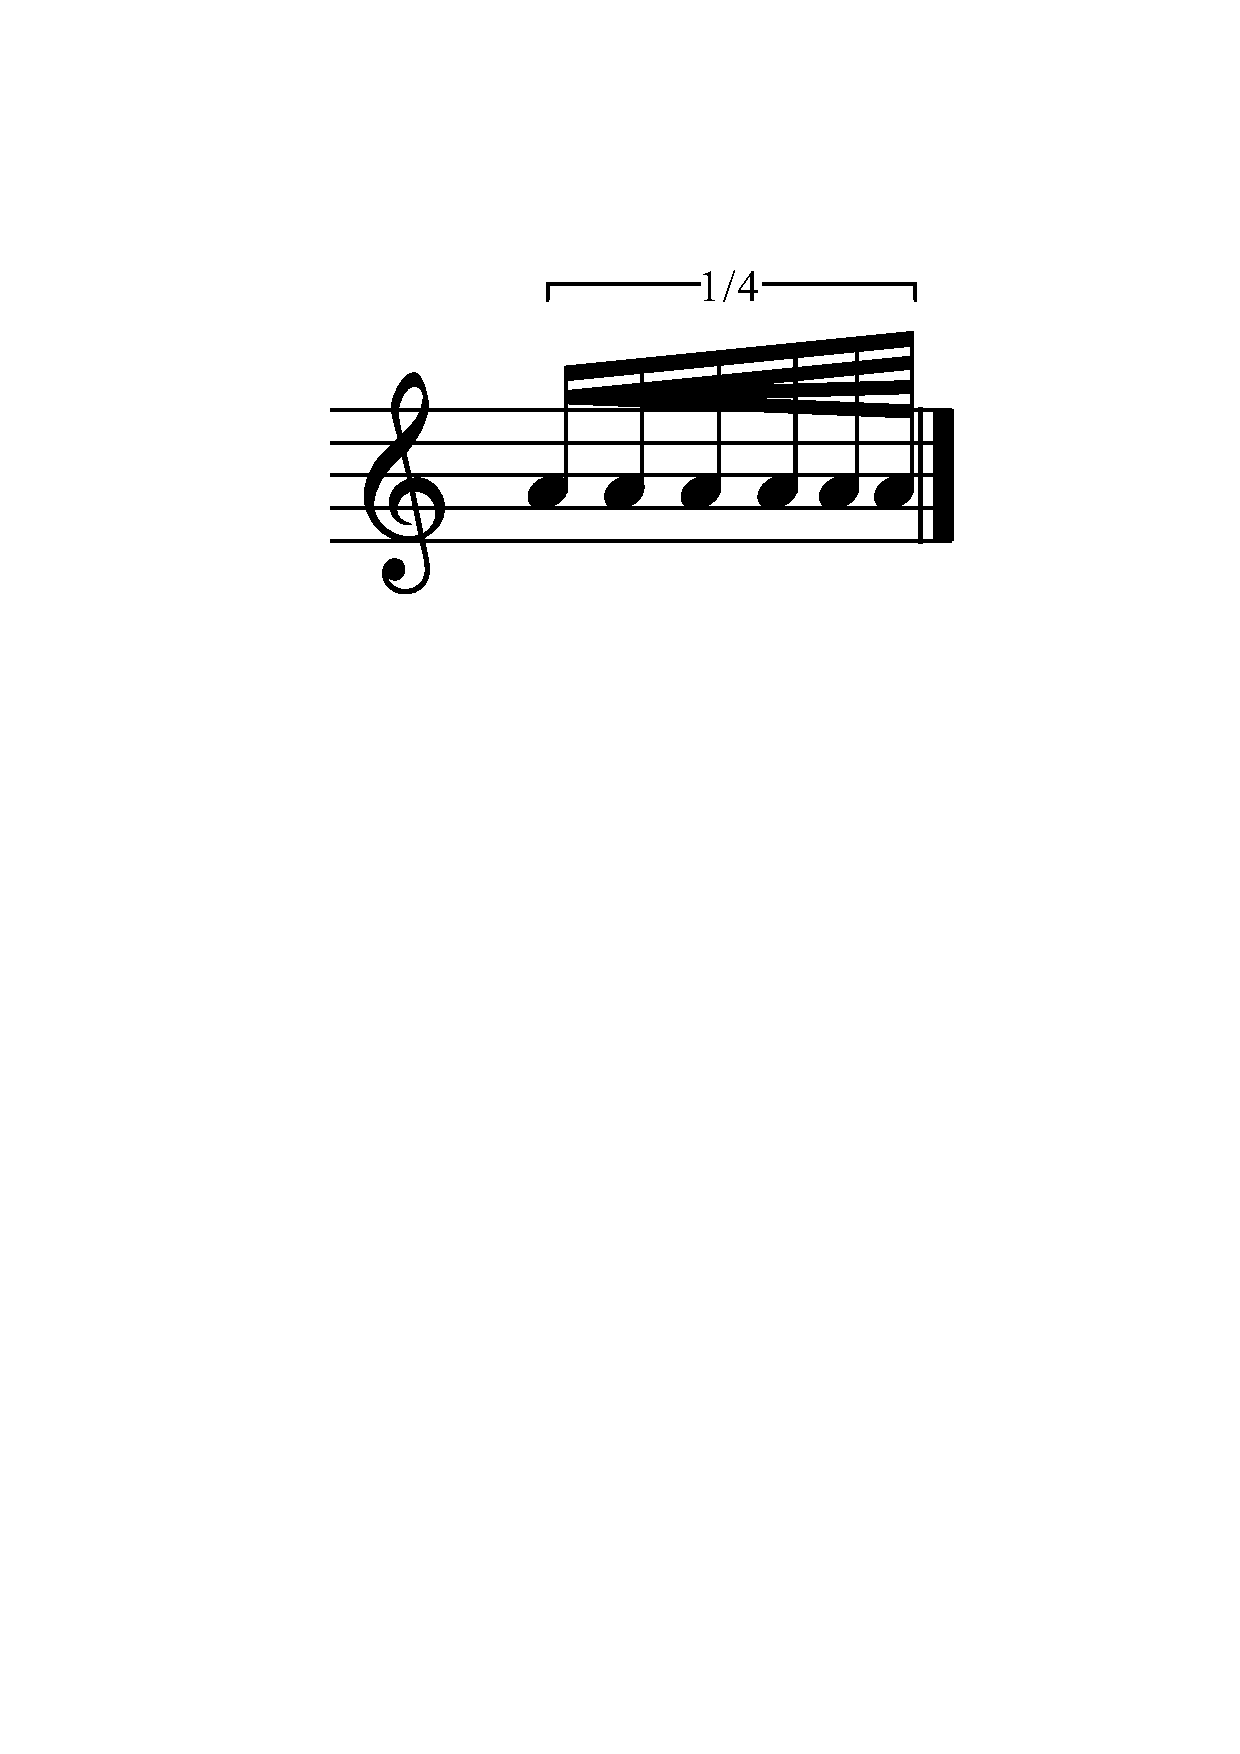
\includegraphics[width=5cm]{img/durationsinternes.pdf}
\caption{Aspect graphique imposé par les durées internes}
\label{fig:interne}
\end{figure}
\end{comment}
%%


\begin{figure}[h]
\centering
\begin{gmncode}
[ 
  \fBeam<durations="1/16,1/64", 
  drawDuration="true">
   (a/8 a/16 a a a/32 a) 
]
\end{gmncode}

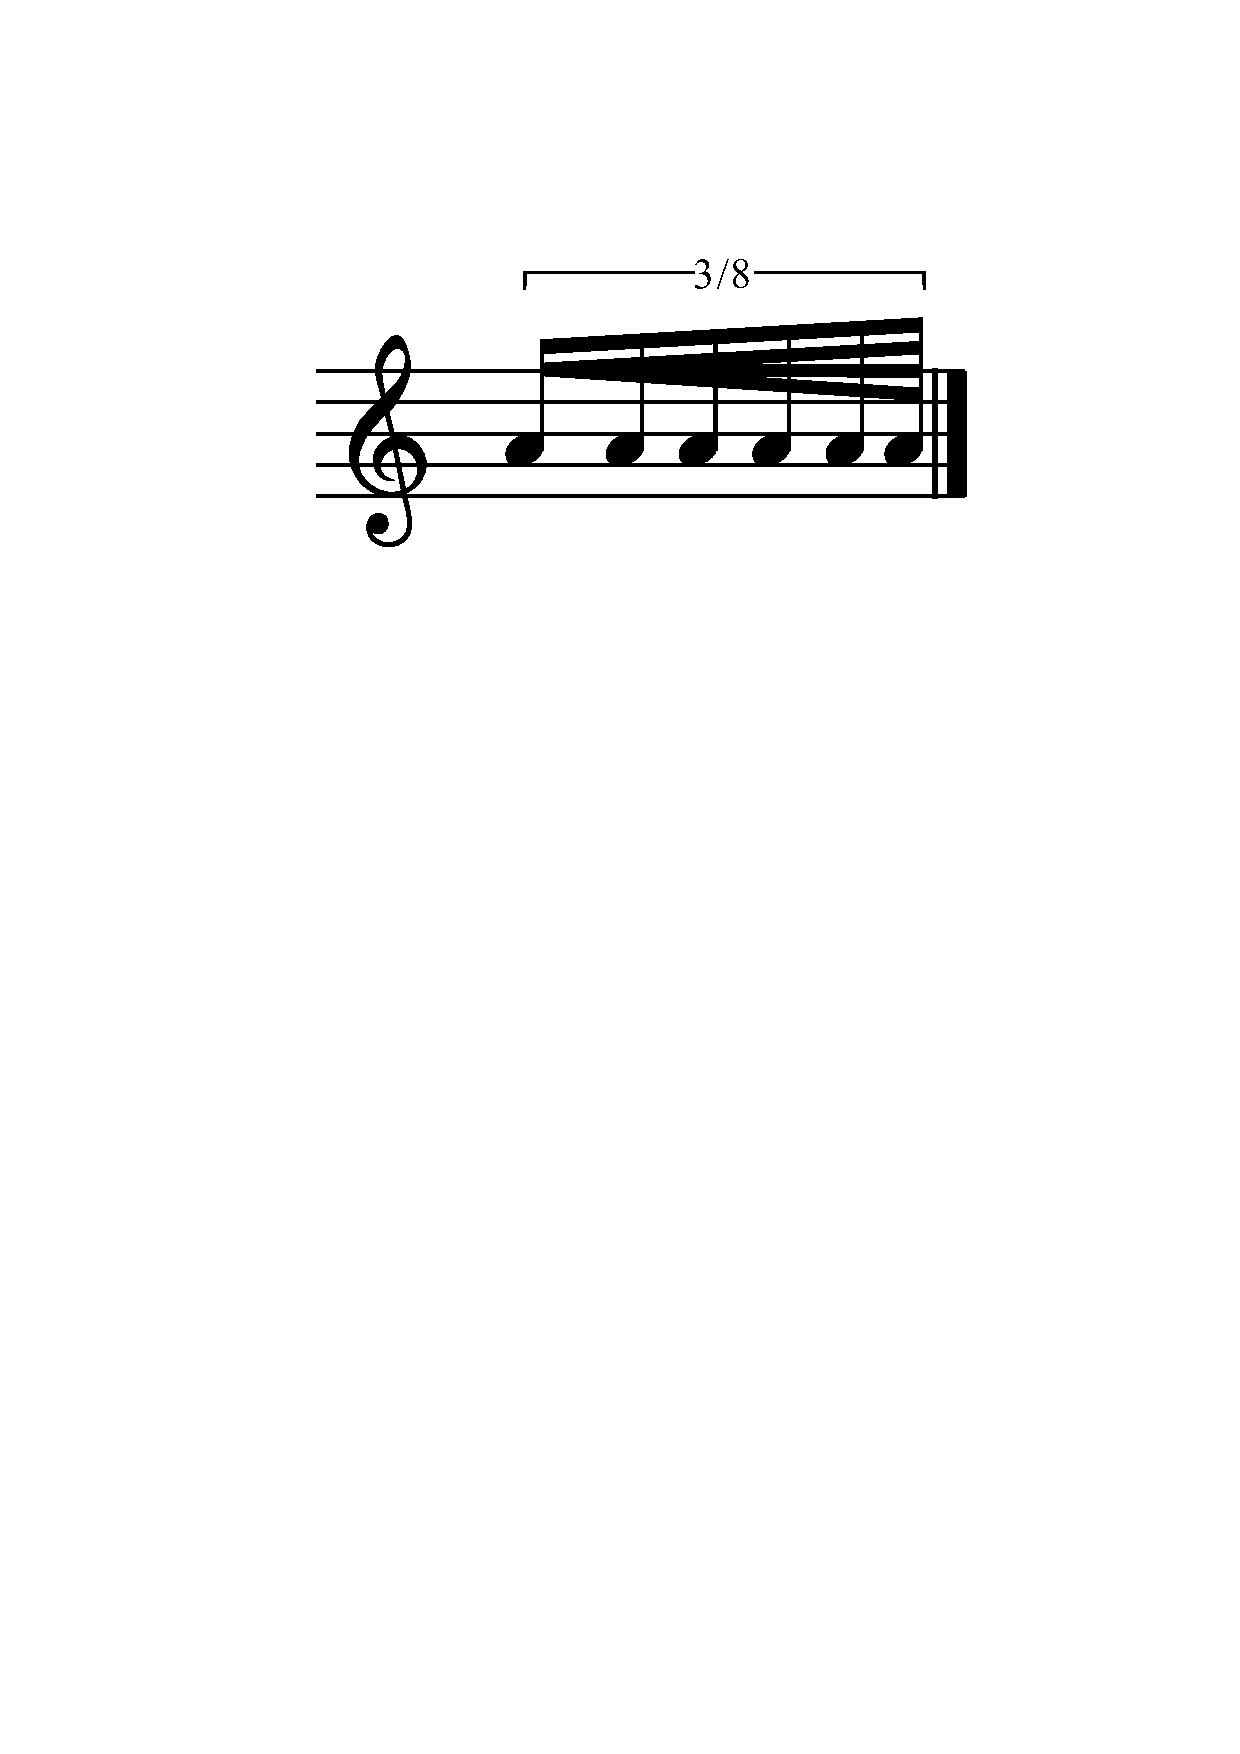
\includegraphics[width=35mm]{img/durations.pdf}
\caption{Aspect graphique imposé par l'utilisateur}
\label{fig:utilisateur}
\end{figure}


% *****************STAFFOFF/ON**********************
\subsection{Tags staffOff / staffOn}\label{subsec:staffoff}

\begin{gmncode}
[ ... \staffOff ... \staffOn ... ]
\end{gmncode}


% littérature ?????????????
% lilypond : même principe, mais les notes et autres éléments se dessinent dans le vide
% permet aussi de passer d'un style de portée à un autre (override staff) ex : 2 lignes...

L'implémentation de ce \emph{tag} vient du besoin de pouvoir faire disparaître et apparaître la partition, en particulier pour cacher une voix muette pendant un certain temps, et donc inutilement dessinée. (Figure \ref{fig:staffoffsimple}) 

Il est cependant généralisé à tous les éléments et toutes les voix de la partition et peut donc être utilisé à la guise et selon les fantaisies de l'utilisateur. (Figure \ref{fig:staffoffexotique})

\begin{figure}[h]
\centering
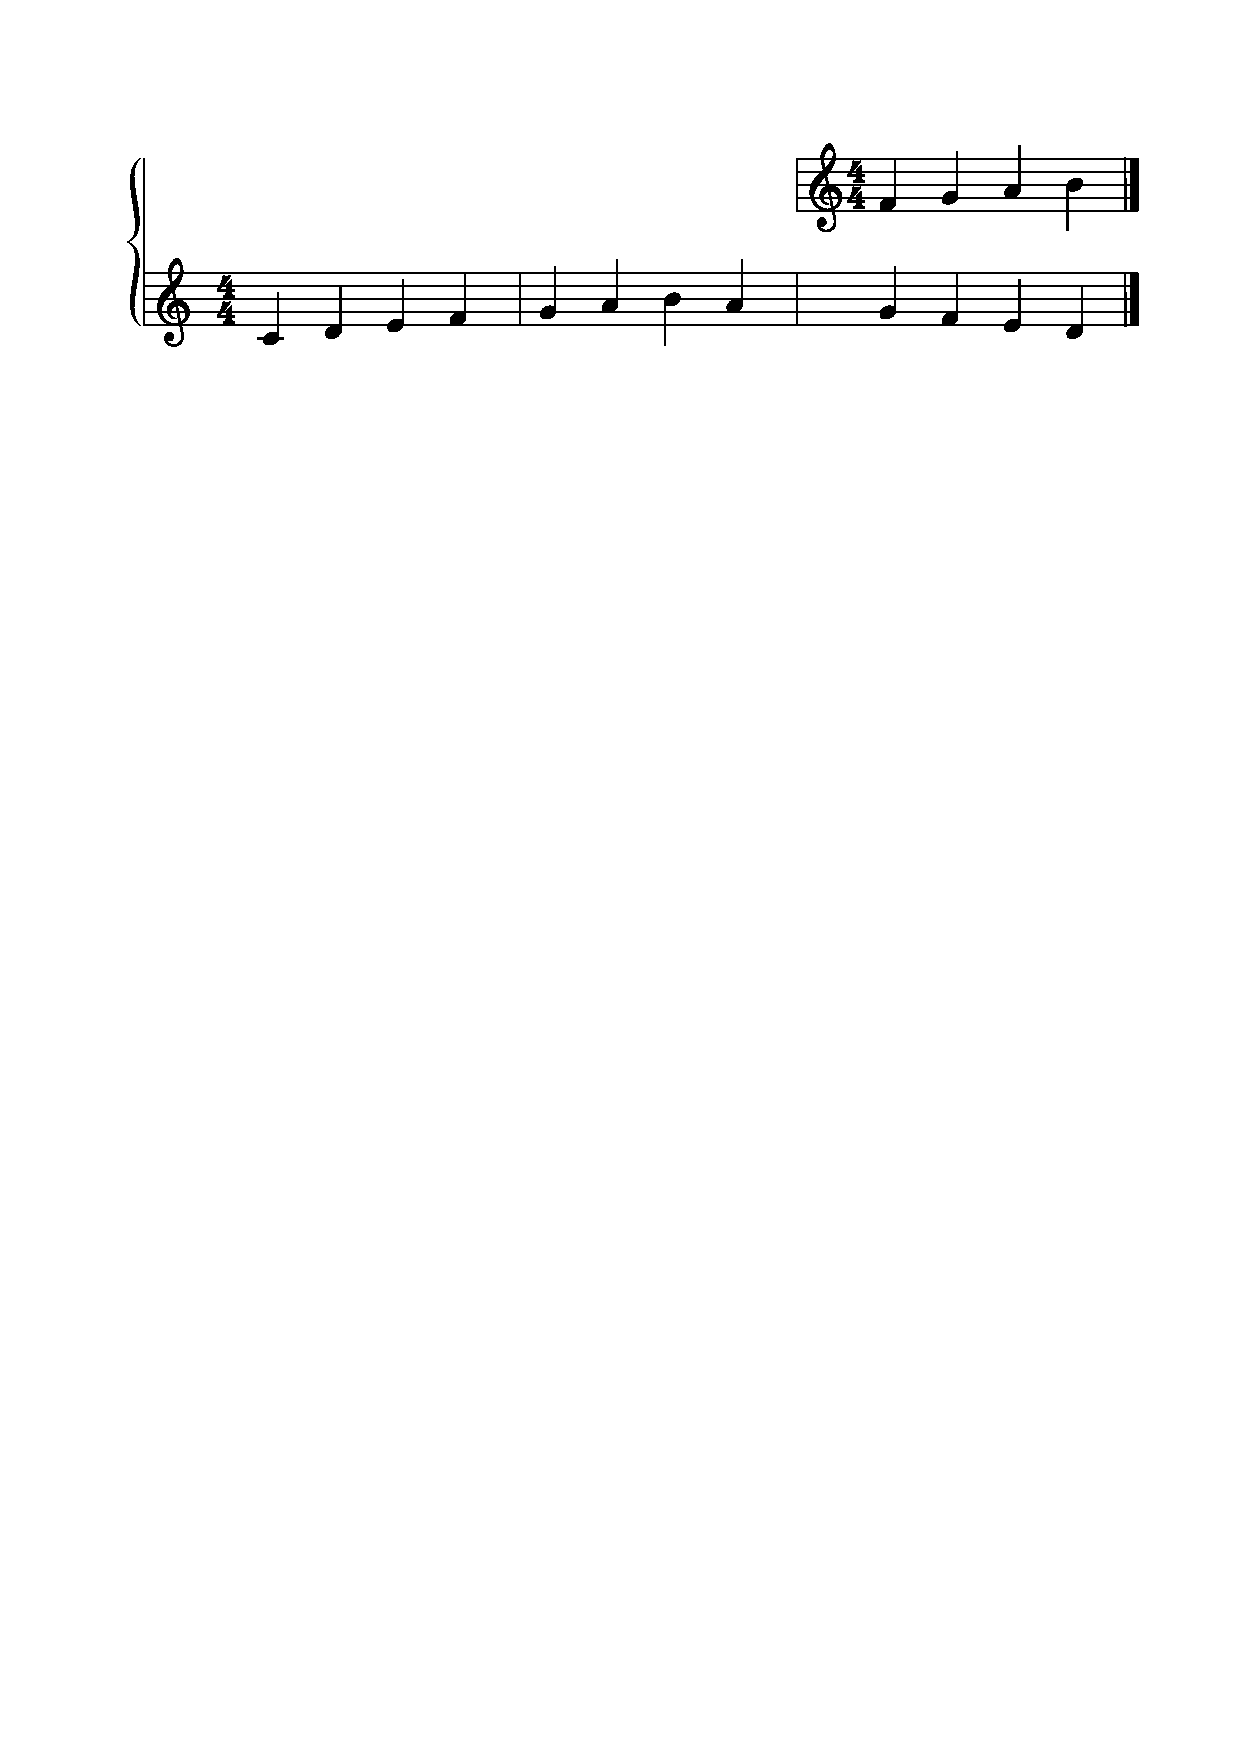
\includegraphics[width=\columnwidth]{img/staffoff.pdf}
\caption{ Exemple \emph{staffOff} classique}
\label{fig:staffoffsimple}
\end{figure}

%{[\meter<"3/4"> a b/2 c \staffOff g/4 e _\staffOn e a/2 \staffOff \slur(e g) \staffOn a b/4 ], [\meter<"3/4"> \staffOff \clef e \staffOn d g \staffOff _/2 g e g \staffOn a b g d/4]}

\begin{figure}[h]
\centering
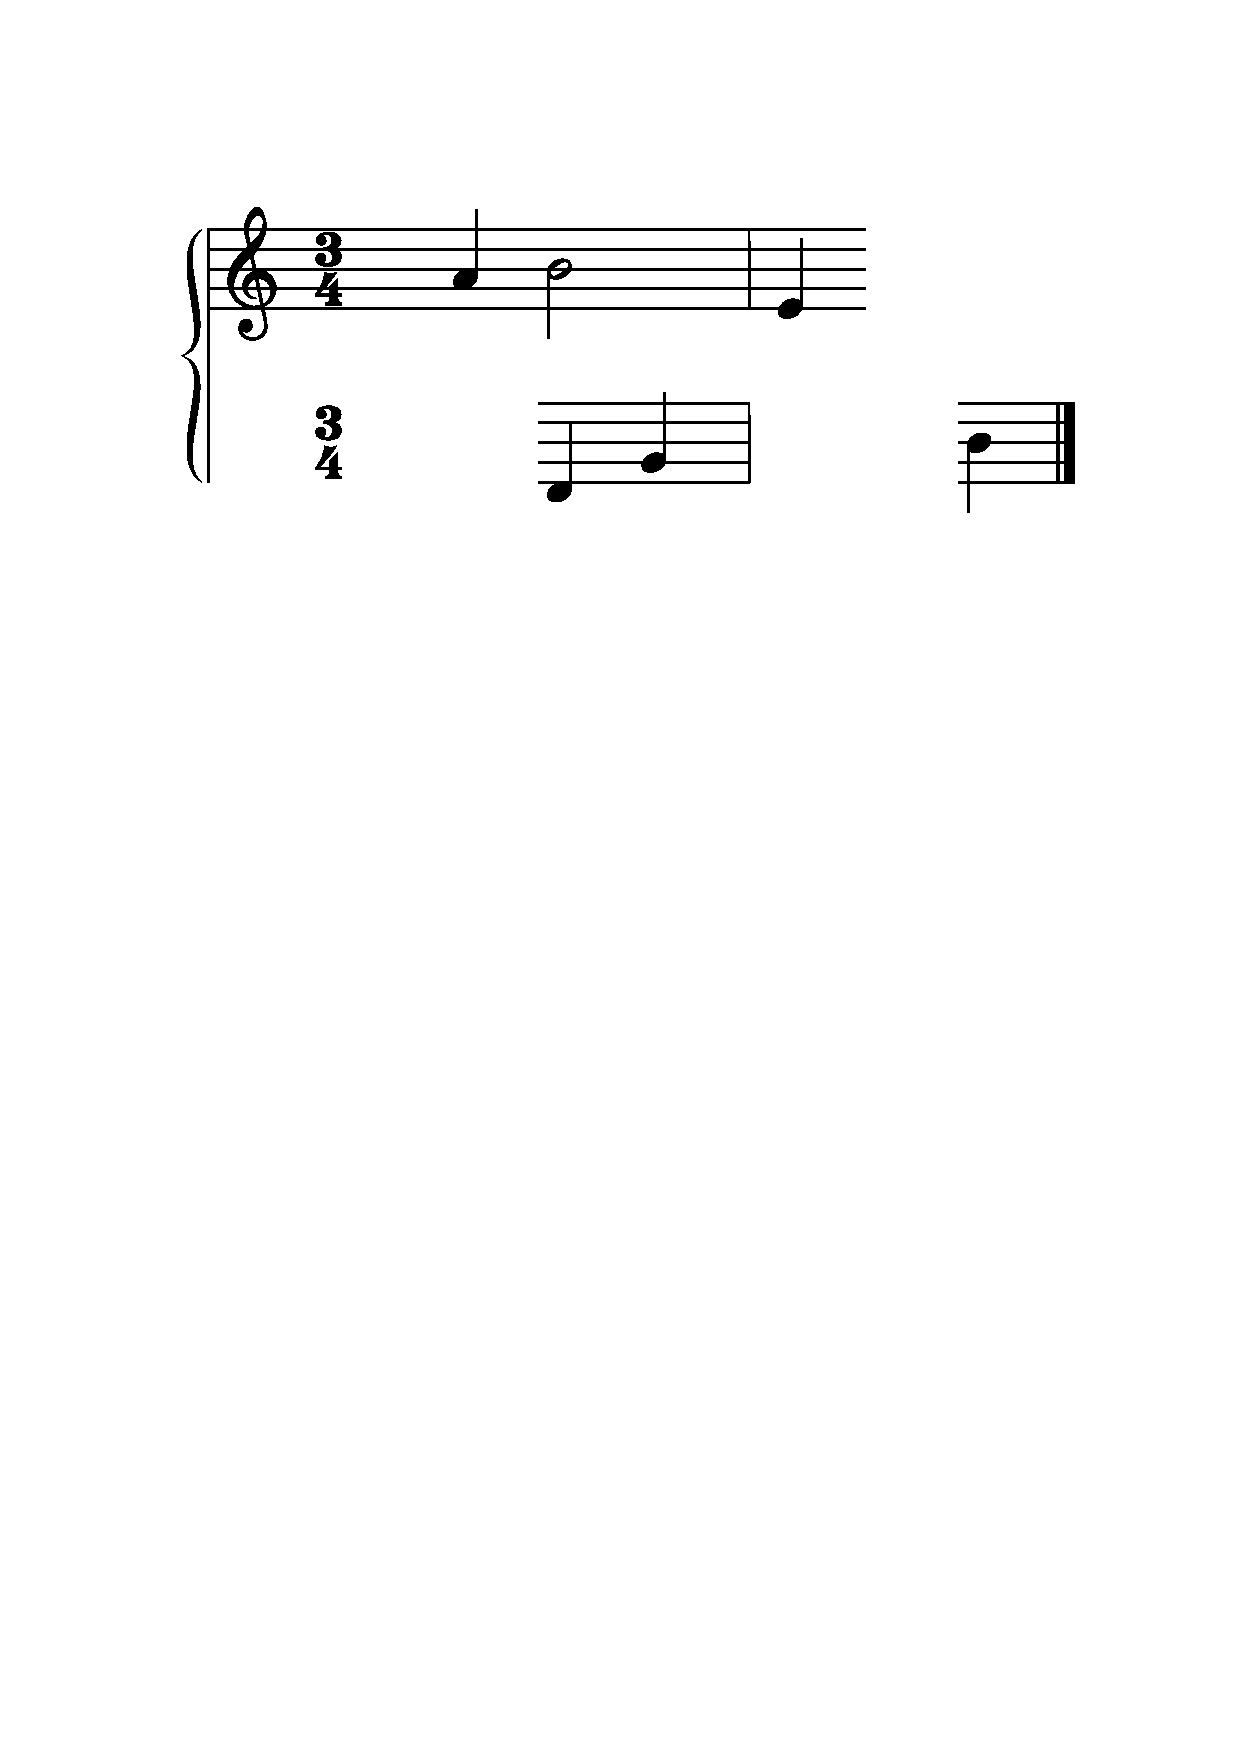
\includegraphics[width=0.8\columnwidth]{img/staffoffexotique.pdf}
\caption{ Exemple \emph{staffOff} plus complexe}
\label{fig:staffoffexotique}
\end{figure}

Il fut important de définir les positions temporelles et graphiques correspondant aux positions dans la description textuelle, en particulier pour les éléments sans durée, dont la position était la même que le \emph{tag}. La solution implémentée consiste à faire disparaître tous les éléments inscrits après le \emph{tag} \emph{\textbackslash{}staffOff} dans la description textuelle, et à préserver ceux décrits avant, même dans le cas d'éléments de durée nulle qui donc pourraient être considérés simultanés à l'arrivée du \emph{tag}. Pour plusieurs éléments simultanés, c'est donc bien l'ordre dans la description textuelle qui indiquera le comportement à adopter. Ainsi, écrire 
% exemple utile ? pertinent sans image ?

\begin{center}
\begin{gmncode}
[\meter<"4/4">\clef\staffOff a b\staffOn c]
\end{gmncode}
\bigskip

n'est pas équivalent à écrire 
\\
\begin{gmncode}
[\staffOff\meter<"4/4">\clef a b\staffOn c]
\end{gmncode} 
\end{center}

Quant à la portée, elle commence, ou s'arrête, aux positions correspondant au début des éléments suivant le \emph{tag}.


%************************ GRAPHIQUES ABSTRAITES ******************
\subsection{Graphiques arbitraires}\label{subsec:graphiquesAbstraites}
\bigskip

\begin{gmncode}
1) \symbol<params>
2) \symbol<params>( notes )
  params : 
    - filePath :
      chemin du fichier
    - position = "top, mid, bot" :
      position de l'image
    - w/h :
      largeur/hauteur de l'image
\end{gmncode}

Une fonctionnalité intéressante manquait dans \guido, la possibilité d'insérer un fichier graphique externe à l'application. Nous avons donc implémenté la possibilité d'appeler dynamiquement une image de type \emph{png}, \emph{jpg} ou \emph{bmp}, à l'aide du \emph{tag} \textbackslash{}\emph{symbol}, et d'ajuster sa taille et sa position dans la partition, afin d'offrir de nouvelles possibilités graphiques à l'utilisateur.

Nous avons séparé en deux les types de symboles:
\begin{itemize}
	\item symbole ne possédant pas de durée mais prenant une certaine place sur la portée, selon sa taille (syntaxe 1);
	\item symbole possédant une durée, et étant alors considéré comme un événement à part entière (syntaxe 2).
\end{itemize}

Pour les deux exemples suivants, les fichiers images sont appelés par un chemin relatif et se situent dans le même répertoire que le fichier \textsc{.gmn} (contenant le code de l'exemple) ouvert.

\exemple\\
Le code suivant produit le résultat présenté en figure \ref{fig:symbol}. Sur la première portée, le symbole ne possède pas de durée, contrairement à la deuxième portée.

\begin{gmncode}
{
  [
    \meter<"4/4"> c f
    \symbol<file="silence.png", dx=-5> 
    c d f
  ],
  [
    \meter<"4/4"> a d
    \symbol<file="ronds.png",
      position="bot"> (f g) g
  ]
}
\end{gmncode}

\begin{figure}[h]
\centering
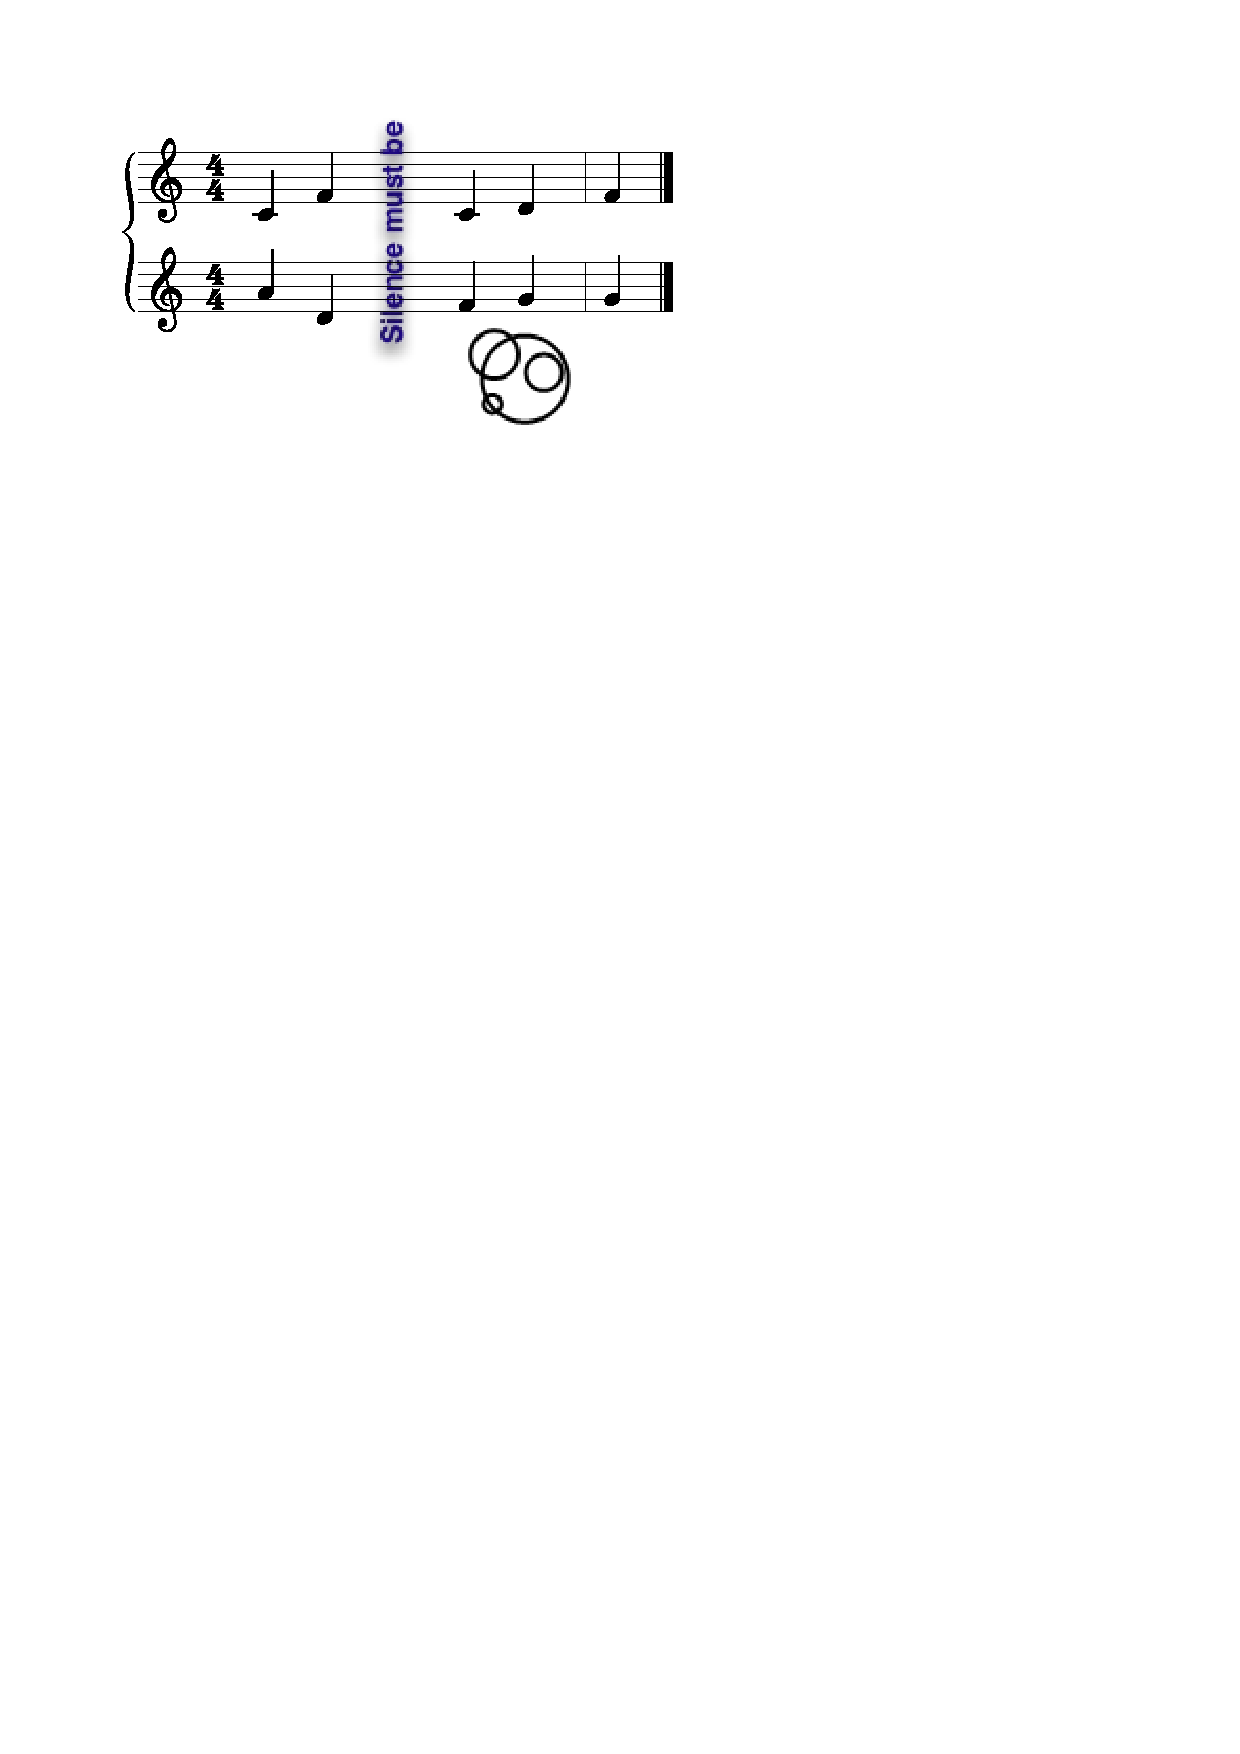
\includegraphics[width=65mm]{img/partitions/symbol.pdf}
\caption{Symboles}
\label{fig:symbol}
\end{figure}

Le chemin du fichier peut être absolu ou bien relatif par rapport au dossier \textsc{home} de l'utilisateur ou par rapport au répertoire contenant le fichier \textsc{gmn} ouvert.

Divers paramètres sont proposés à l'utilisateur pour gérer l'affichage de son symbole:
\begin{itemize}
	\item \textsc{position} (\emph{top}, \emph{mid} ou \emph{bot}), positionnant l'image par rapport à la portée;
	\item \textsc{size}, correspondant à sa taille;
	\item \textsc{w/h}, permettant de régler la largeur et la hauteur de l'image;
	\item \textsc{dx/dy}, insérant un offset horizontal ou vertical.
\end{itemize}

%************************ AMELIORATIONS DIVERSES ******************
\subsection{Améliorations diverses}\label{subsec:amelioraions}


%*****************TRILLES********************
\subsubsection{Trilles}\label{subsubsec:trilles}

% littérature
% lilypond : e\trill f\trill ... sans vaguelette sinon \startTrillSpan ... \stopTrillSpan
%\gardner Read

\begin{gmncode}
\trill<param-list>(chord-series)
\end{gmncode}

% Citation wiki
Un \emph{trille} est \og{}un ornement musical qui consiste à alterner très rapidement la note de base (la note principale), sur laquelle est noté le \emph{trille}, et la note située juste au-dessus\fg{}.

Dans la version précédente de \guido, le \emph{trille} à proprement parler n'était indiqué que par le symbole \textit{\textbf{tr}} placé au dessus de la note. Il paraissait pourtant important que la notation comprenne également la ligne ondulée du \emph{trille} qui suit celui-ci et en indique la durée. Comme ce symbole était déjà en partie implémenté, il fallait pouvoir lui offrir plus de souplesse sans pour autant en complexifier la notation.

%D'après Elaine Gould \cite{gould2011behind}, la ligne du \emph{trille} doit être dessinée depuis le signe \textit{\textbf{tr}} jusqu'au début du prochain évènement (la prochaine note ou le prochain soupir), sauf si celui-ci se situe directement après la prochaine barre de mesure, la ligne s'arrêtant dans ce cas à la barre elle-même. 

% justifier l'intérêt de tr et anchor ?
De plus, nous avons voulu donner la possibilité de choisir de dessiner ou non le signe \textit{\textbf{tr}}, ainsi que de pouvoir changer l'ancrage de la ligne pour le déplacer sur la tête de la note. Cela fut implémenté grâce au \emph{param} \emph{tr} qui accepte comme valeurs "true" ou "false" et \emph{anchor} qui accepte comme valeurs "note" ou "tr" (Figure \ref{fig:trillanchor}). Le reste des modifications graphiques pouvant être effectuées manuellement par l'utilisateur à travers les paramètres classiques de déplacement (\textit{dx}, \textit{dy}), de couleur (\textit{color}), et de taille (\textit{size}).

\begin{figure}[h]
\centering
\begin{gmncode}
[ \trill<tr="false", anchor="note">
( {g} {a/2} ) ]
\end{gmncode}
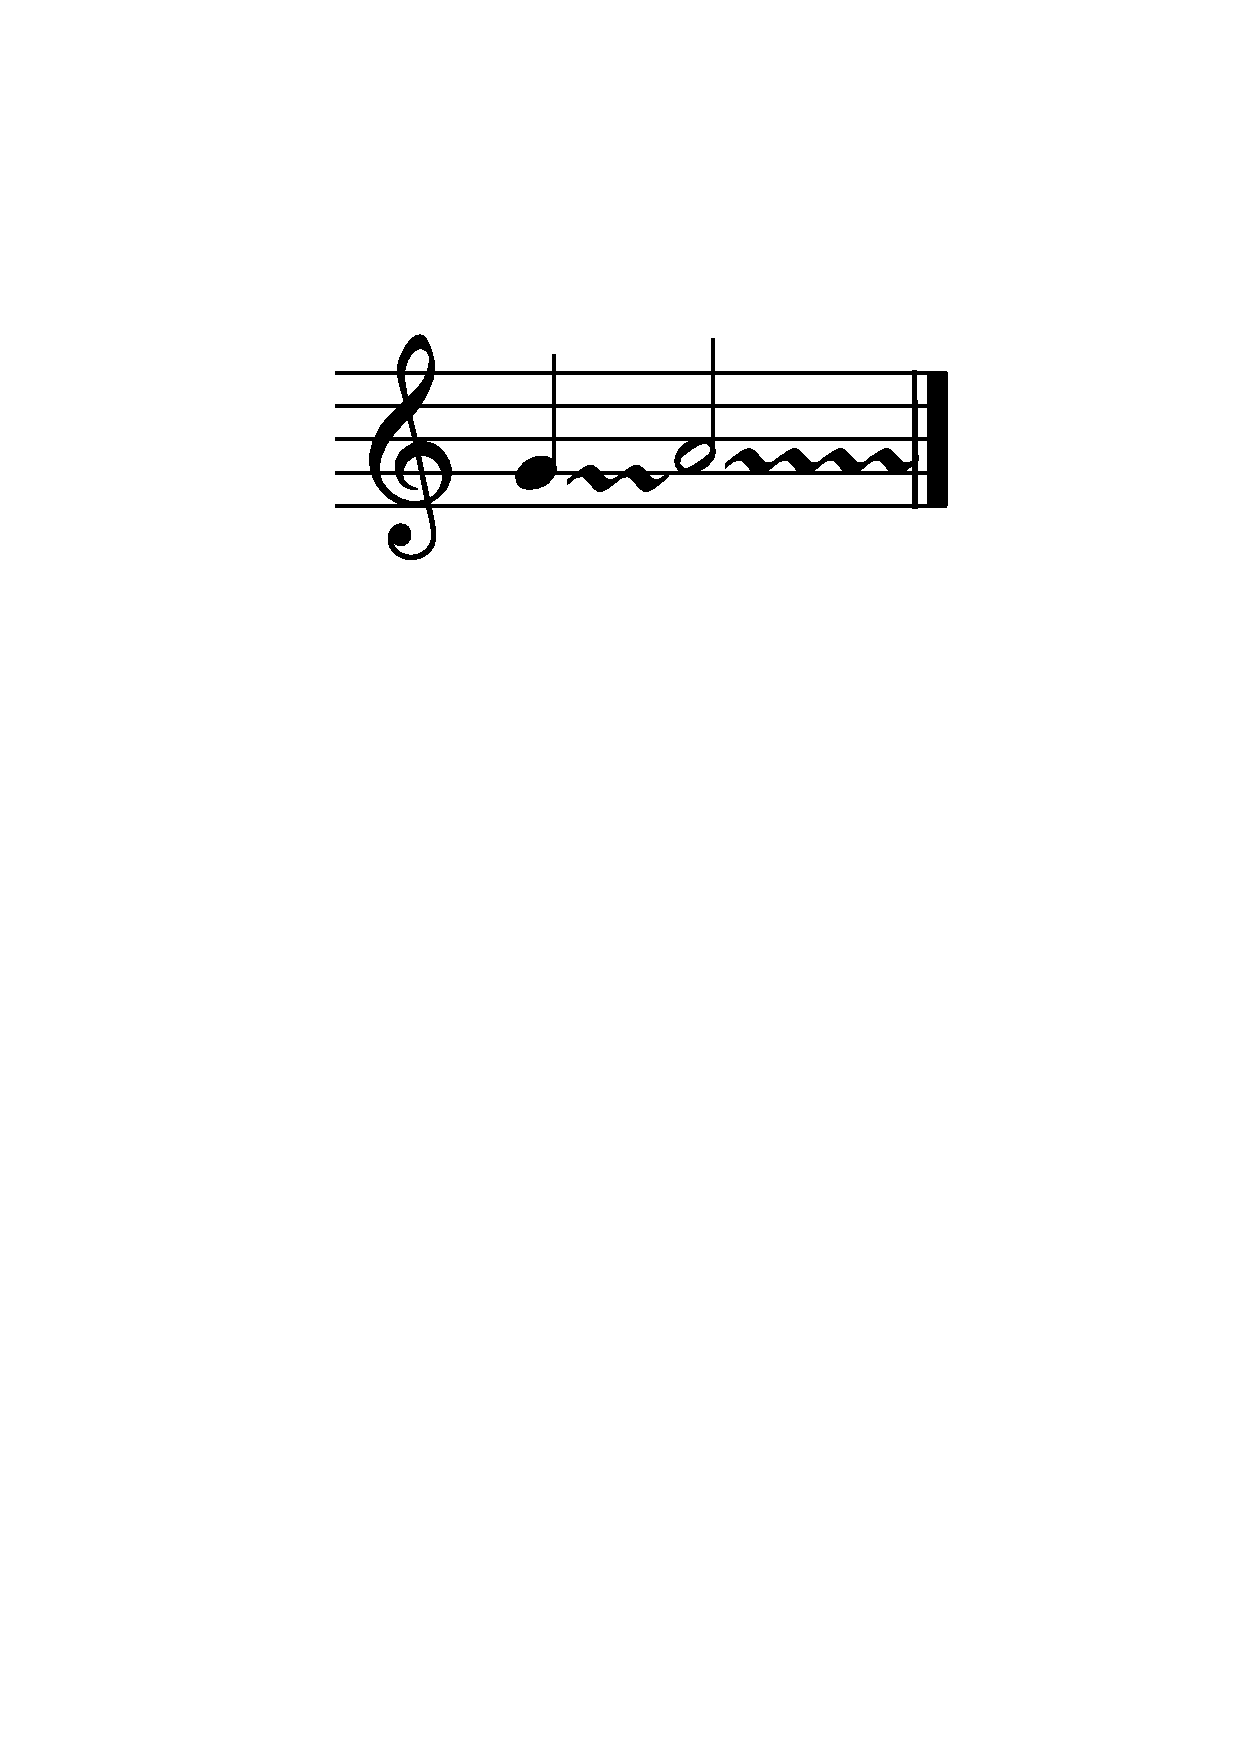
\includegraphics[width=30mm]{img/trillanchor.pdf}
\caption{Cas du \emph{trille} ancré à la tête de note, et \textit{\textbf{tr}} optionnel}
\label{fig:trillanchor}
\end{figure}

%************************* NOUVEAUX ATTRIBUTS **************************
\subsubsection{Nouveaux attributs}\label{subsubsec:attributs}

% colas /////////////


%%%%%%%%%%%%%%%%%%%% CONTROLE DE RENDU %%%%%%%%%%%%%%%%%
\section{Contr\^ole de rendu}\label{sec:controleRendu}

%*************************GLISSANDI ET ACCORDS*******************************
\subsection{Glissandi et accords}\label{subsec:glissandiAccords}

Concernant le \emph{glissando}, une certaine flexibilité devait être trouvée quant au rendu graphique d'un \emph{glissando} entre les différentes notes de deux accords, ne possédant eux-mêmes pas forcément le même nombre de notes. La solution proposée est celle qui nous a paru la plus intuitive : l'utilisateur choisit quelle note du premier accord sera liée avec quelle note du second. Pour ce faire, il lui suffit de les écrire dans l'ordre, c'est à dire : la première note de l'accord A sera liée à la première note de l'accord B, la seconde de A à la seconde de B\dots{}(Figure \ref{fig:glissandosimple})

\begin{figure}[h]
\begin{center}
\begin{gmncode}
[\glissando({e,a} {f,b} {a,d})]
\end{gmncode}
\bigskip

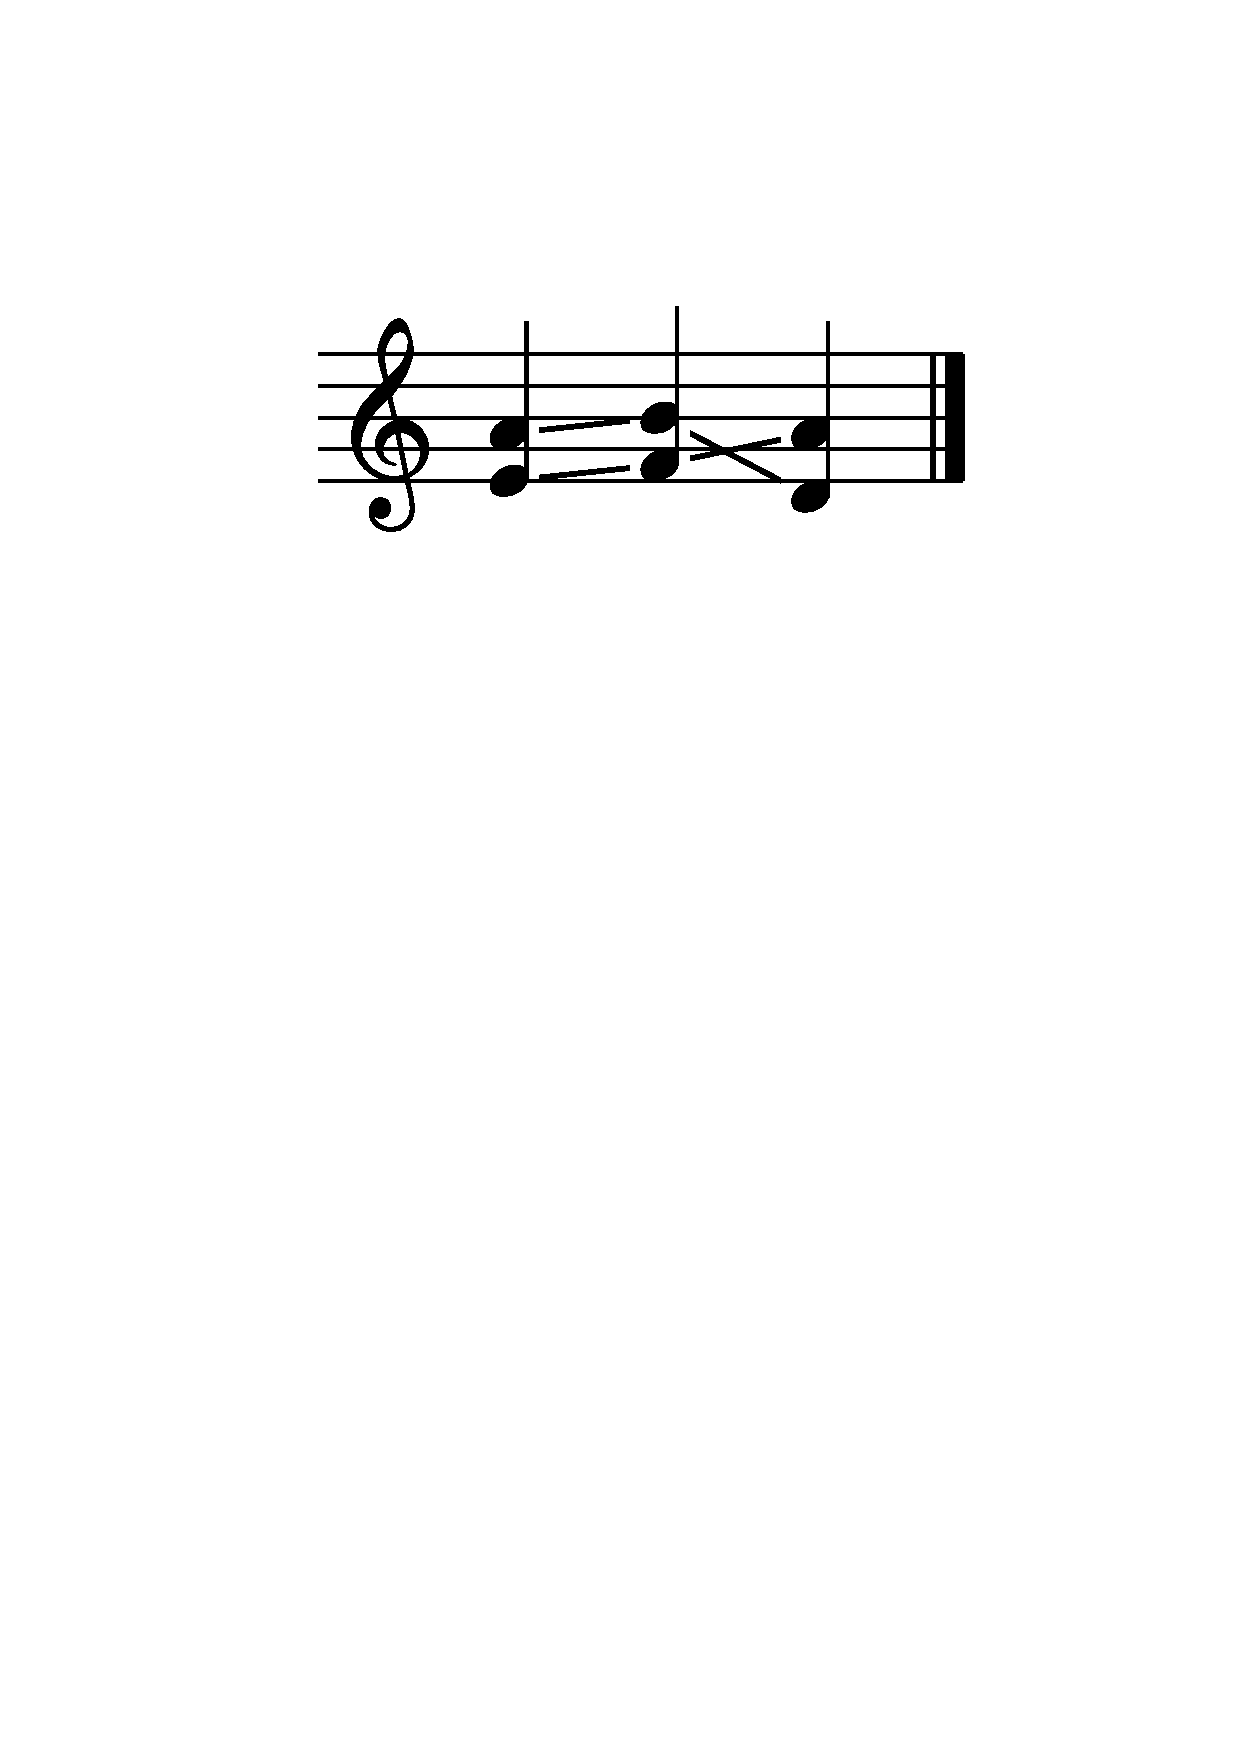
\includegraphics[width=35mm]{img/glissandosimple.pdf}
\caption{\emph{glisandi} entre accords}
\label{fig:glissandosimple}
\end{center}
\end{figure}

L'unique problème avec ce choix peut se poser lors d'un conflit dans l'ordre imposé par le glissando précédent et par le suivant, comme dans le premier cas de l'exemple Figure \ref{fig:glissandopb}. Il est alors possible de faire appel à une seconde voix, et au \emph{tag \textbackslash{}staff \textless{}numero de portée\textgreater{}} qui pourra créer sur une même portée d'autres glissandi en parallèle et indépendants des premiers (Figure \ref{fig:glissandopb}).


\begin{figure}[h]
\centering
\begin{gmncode}
[ \glissando(e {d,f,a} g) b ]
\end{gmncode}
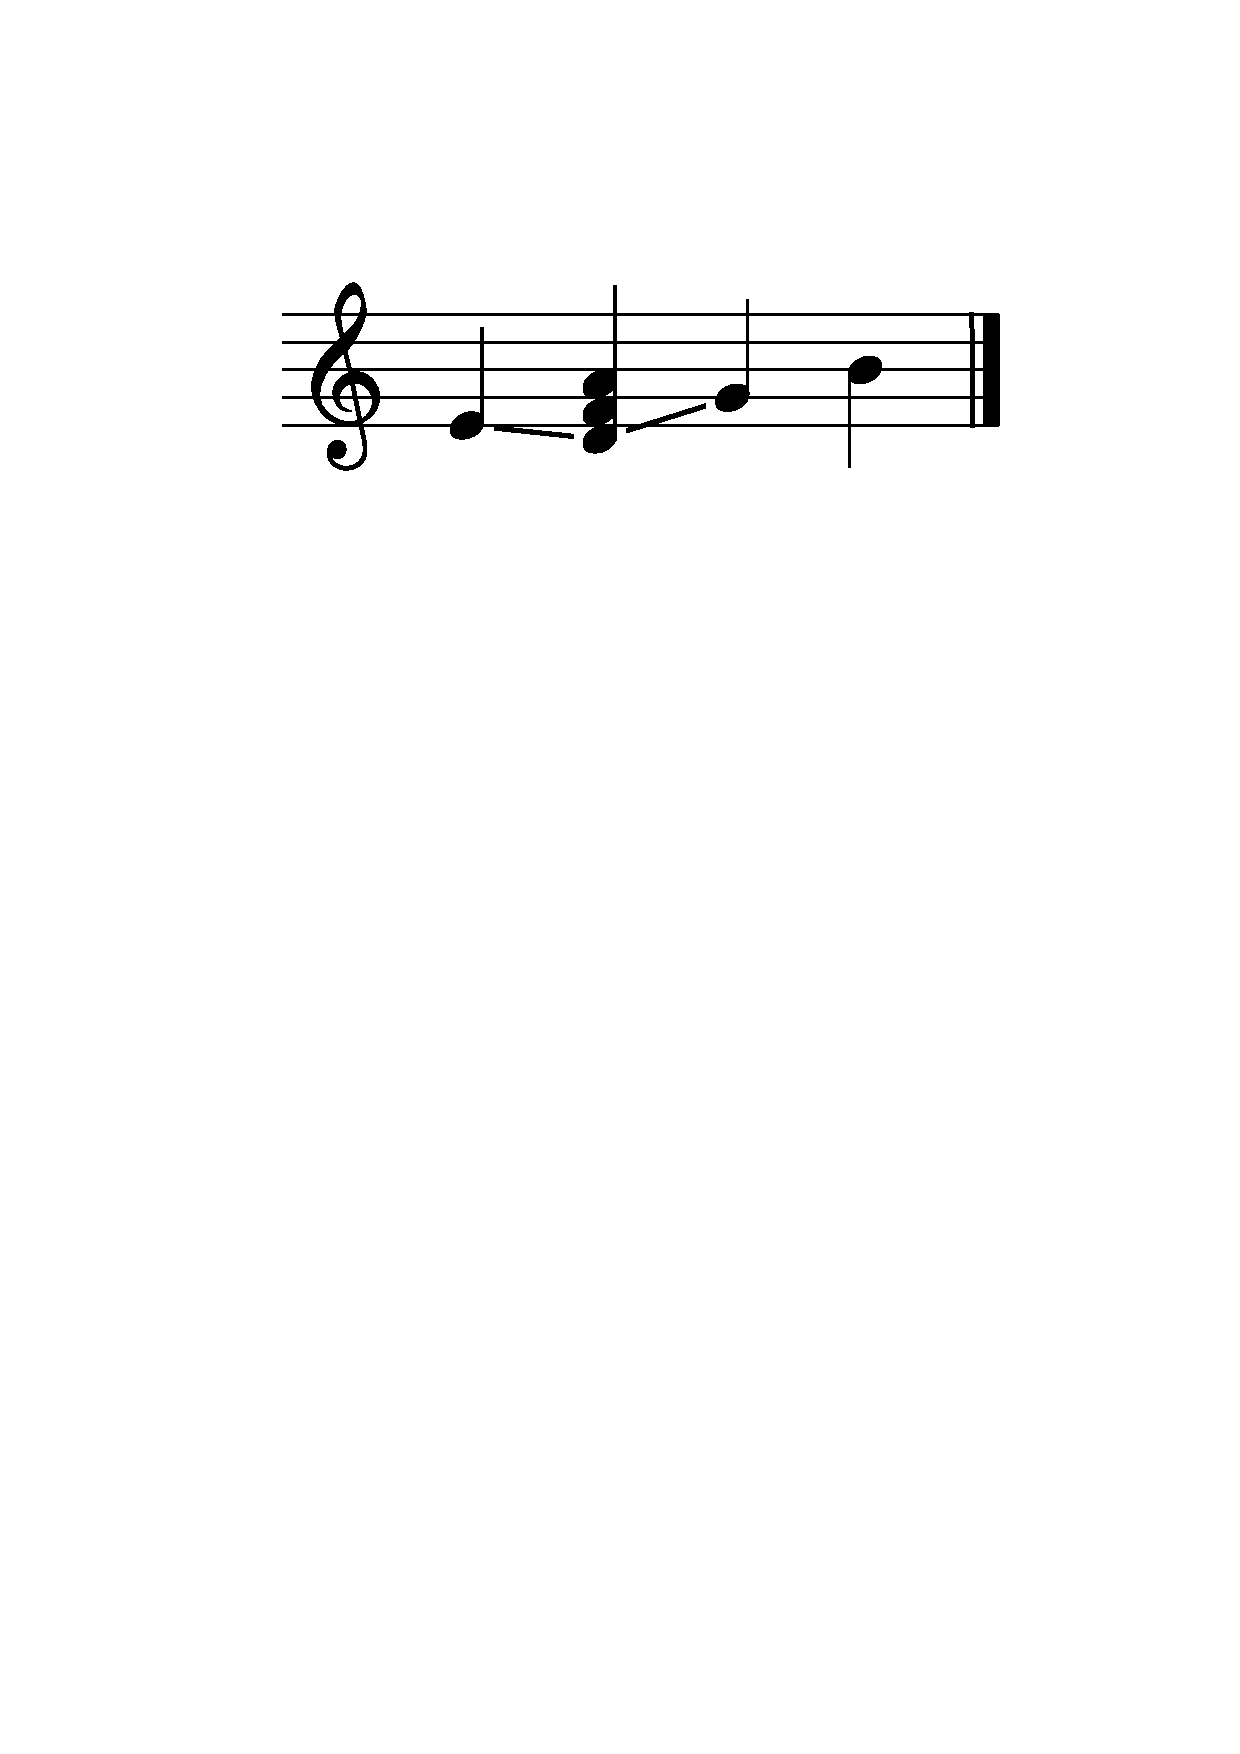
\includegraphics[width=4cm]{img/glissandopb.pdf}

\begin{gmncode}
{ 
  [ \glissando( e {d,f}) empty b ],
  [ \staff<1> empty \glissando( a g ) empty ] 
}
\end{gmncode}
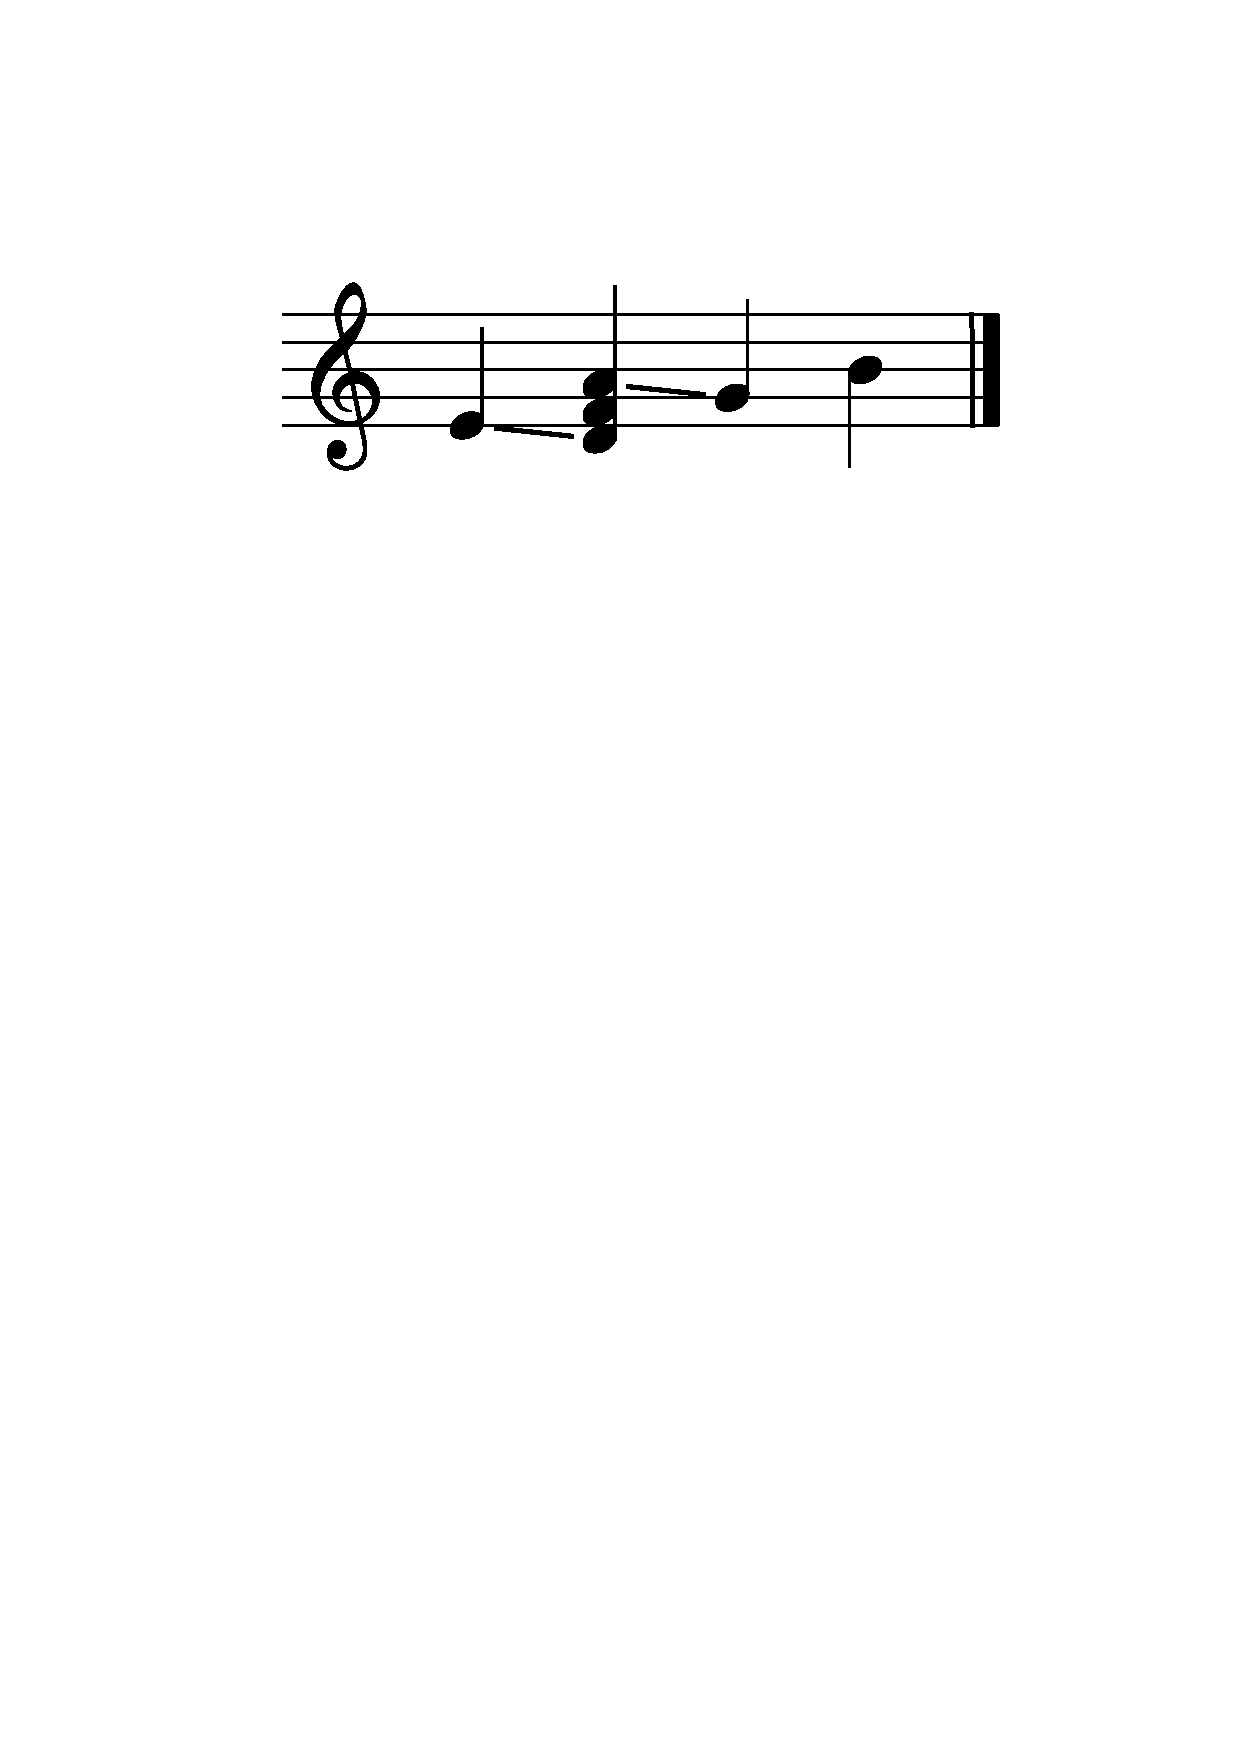
\includegraphics[width=4cm]{img/glissandosanspb.pdf}
\caption{Cas de recours à une seconde voix pour le \emph{glissando} -
'empty' représente une note vide.}
\label{fig:glissandopb}
\end{figure}


%*****************************TRILLES ET TIES****************************************
\subsection{Trilles et liaisons}\label{subsec:trillesLiaison}

Au niveau du trille, une subtilité au niveau du contr\^ole du rendu a également été ajoutée. Il fallait définir le comportement quant aux notes liées, soit de manière automatique de par la présence d'une barre de mesure, soit de manière explicitement décrite par l'utilisateur. La solution adoptée est de dessiner la ligne de \emph{trille} jusqu'à la fin de la dernière note liée si celle-ci provient d'une note plus longue découpée automatiquement, mais de s'arrêter normalement à la prochaine note si la liaison a été explicitée par l'utilisateur, qui pourra alors décider de répéter le \emph{trille} sur cette autre note, ou non. (Figure \ref{fig:trill})

\begin{figure}[h]
\centering
\begin{gmncode}
{
  [\meter<"2/4"> \trill({a} {a/2})],
  [\meter<"2/4"> \trill({a} \tie({a} {a}))]
}
\end{gmncode}
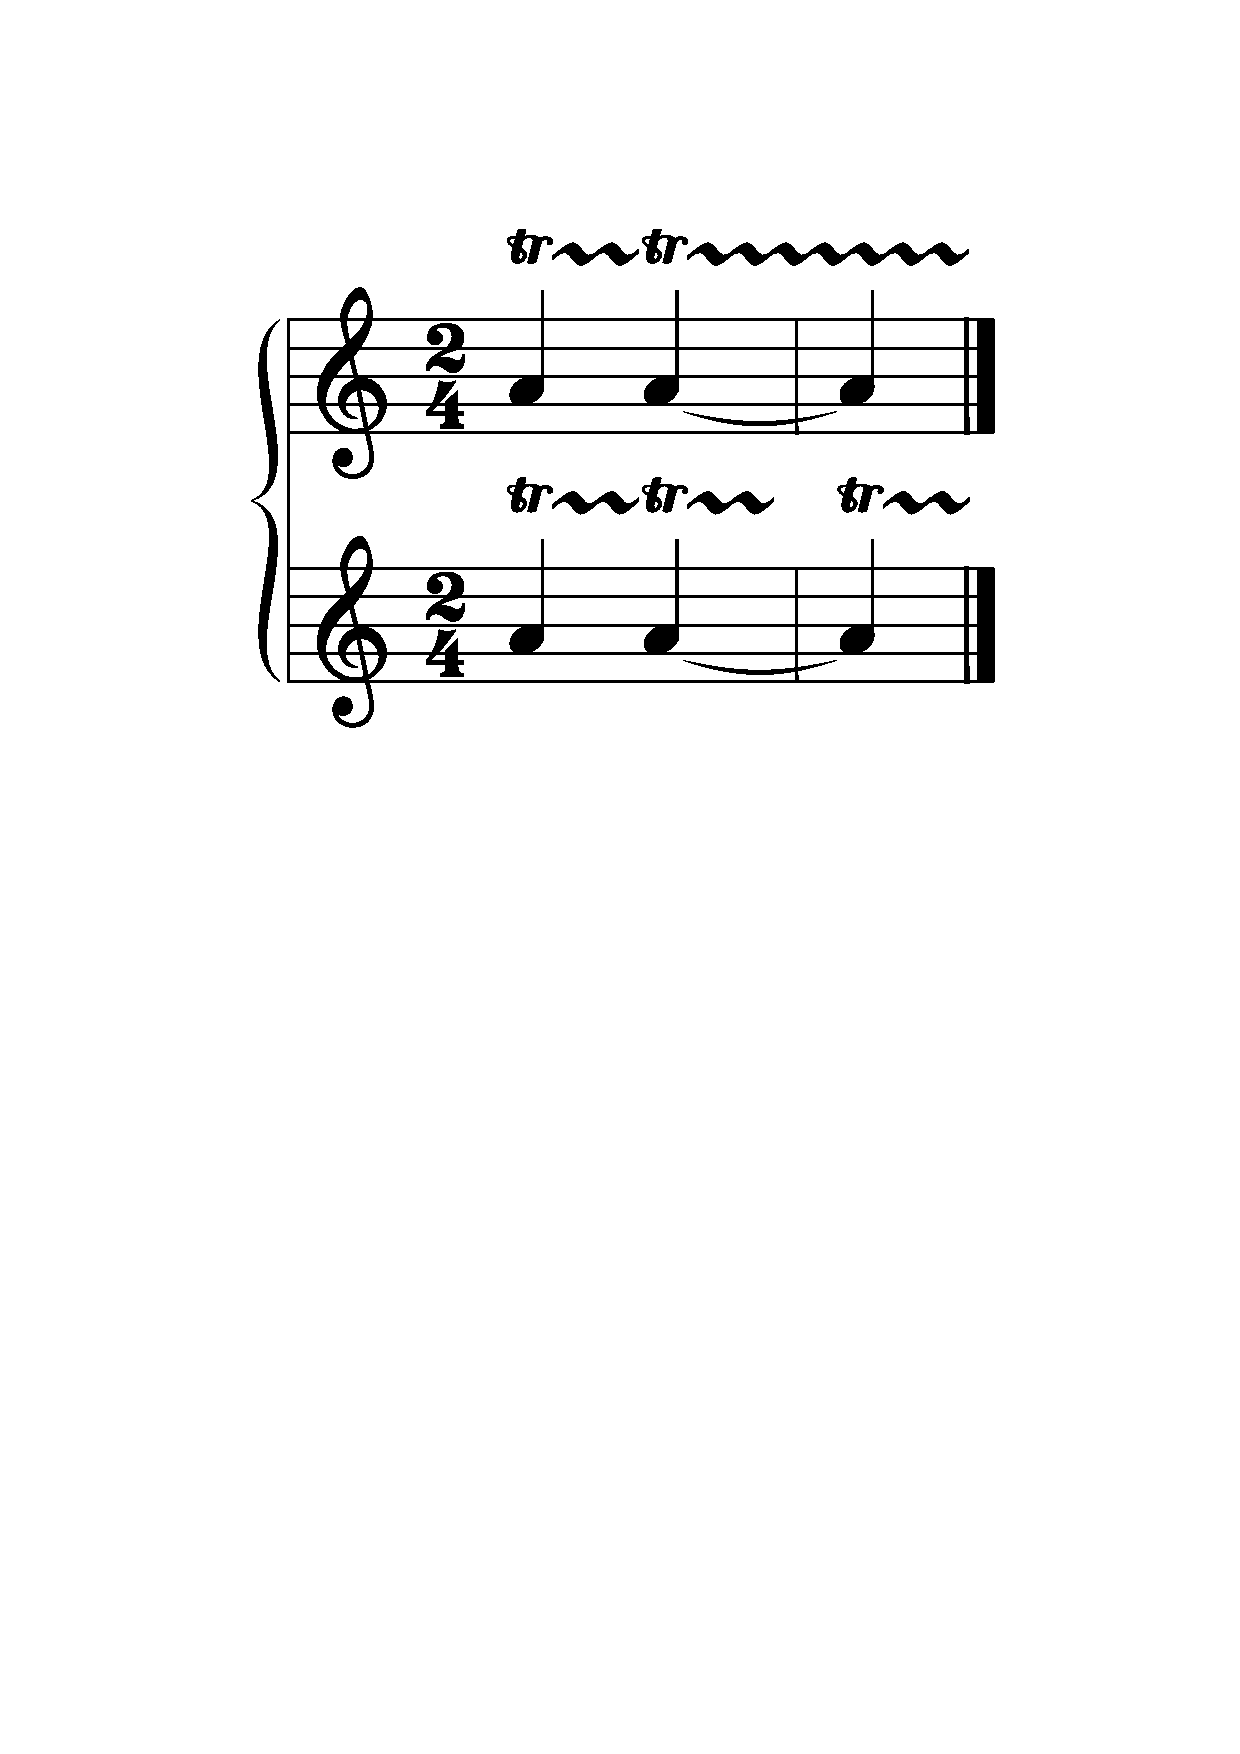
\includegraphics[width=45mm]{img/trill.pdf}
\caption{Cas du \emph{trille} appliqué à des notes liées}
\label{fig:trill}
\end{figure}

%%%%%%%%%%%%%%%%%%%% COMBINAISONS %%%%%%%%%%%%%%%%%
\section{Combinaisons}\label{sec:combinaisons}

%*****************************GLISSANDI ET CLUSTERS****************************************
\subsection{Glissandi et clusters}\label{subsec:glissandiCluster}

Lors de combinaisons de \emph{glissandi}  avec des accords ou des \emph{clusters}, il nous a paru intéressant, comme on peut le voir dans \cite{gould2011behind} (p.143) ou dans \cite{stone1980music} (p.61), de donner la possibilité de remplir l'espace entre ces \emph{glissandi} grâce à un \emph{param} \emph{fill}. Une certaine flexibilité peut être trouvée dans le dessin grâce aux \emph{params} graphiques \emph{dx1}, \emph{dx2}, \emph{dy1}, \emph{dy2}, ainsi que \emph{thickness} qui permettent de modifier l'aspect du \emph{glissando}. (Figure \ref{fig:glissandofill})

\begin{figure}[h]
\begin{center}
\begin{gmncode}
[ 
  \glissando<fill="true", dx1=-2, dx2=2, 
   thickness=2.2>(\cluster({e,g} {c,b}))
  \glissando<fill="true">({c,e,g} {a,c2,f1}) 
]
\end{gmncode}

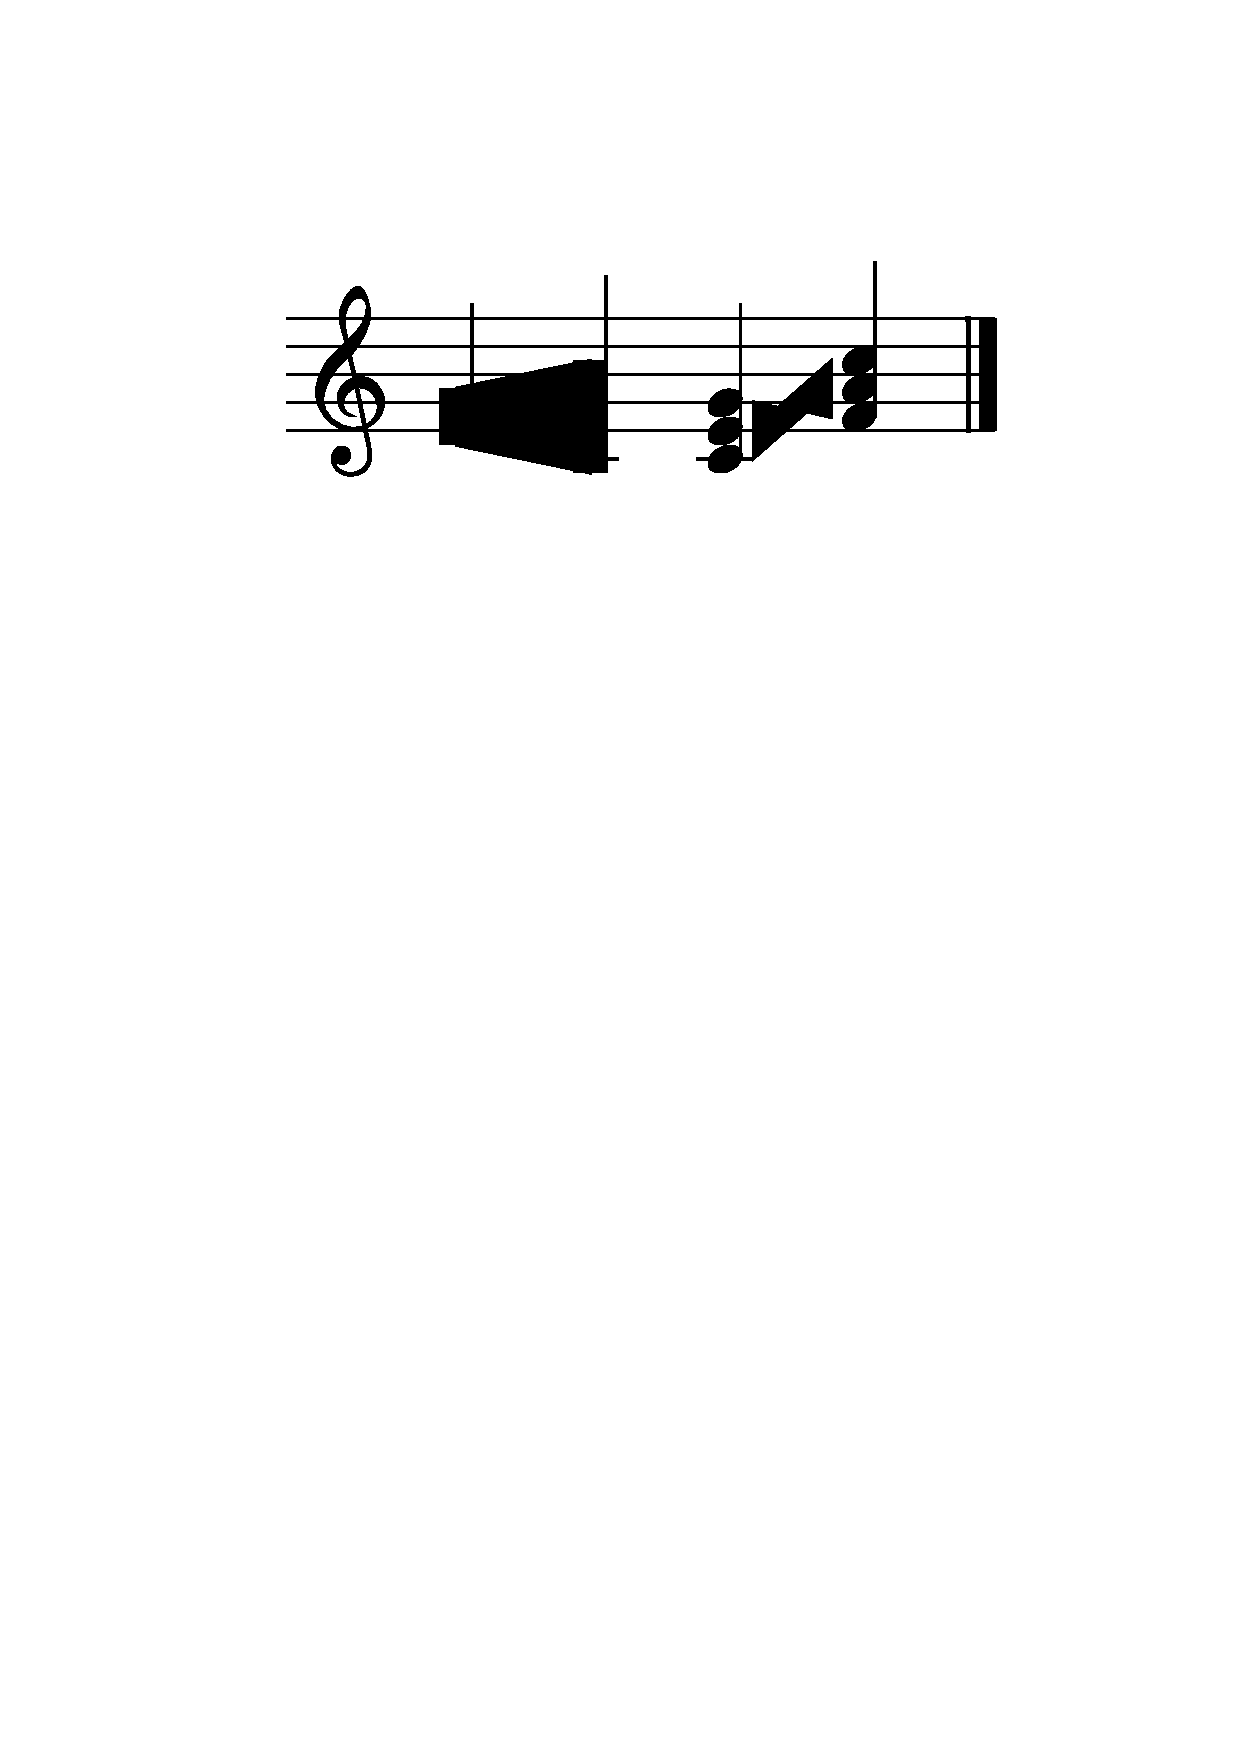
\includegraphics[width=4cm]{img/glissandofill.pdf}
\caption{\emph{glissandi} entre accords et clusters avec \emph{param} de remplissage}
\label{fig:glissandofill}
\end{center}
\end{figure}

%*****************************HIERARCHIE BEAMS****************************************
\subsection{Combinaisons de beams}\label{subsec:combinaisonBeams}

% justification des hierarchies de beams ?
Enfin, concernant le \emph{feathered beam} comme le \emph{beam} classique, il est maintenant possible de créer des hierarchies de \emph{beams} : c'est à dire d'englober plusieurs \emph{beams} dans un plus grand, afin de les joindre par une barre principale commune (Figure \ref{fig:fbeamhierarchie}).

\begin{figure}[h]
\centering
\begin{gmncode}
[ 
  \beam( 
    \fBeam(c/8 e d f g/32) 
    \fBeam(a/16 f e d c/64) 
  ) 
]
\end{gmncode}

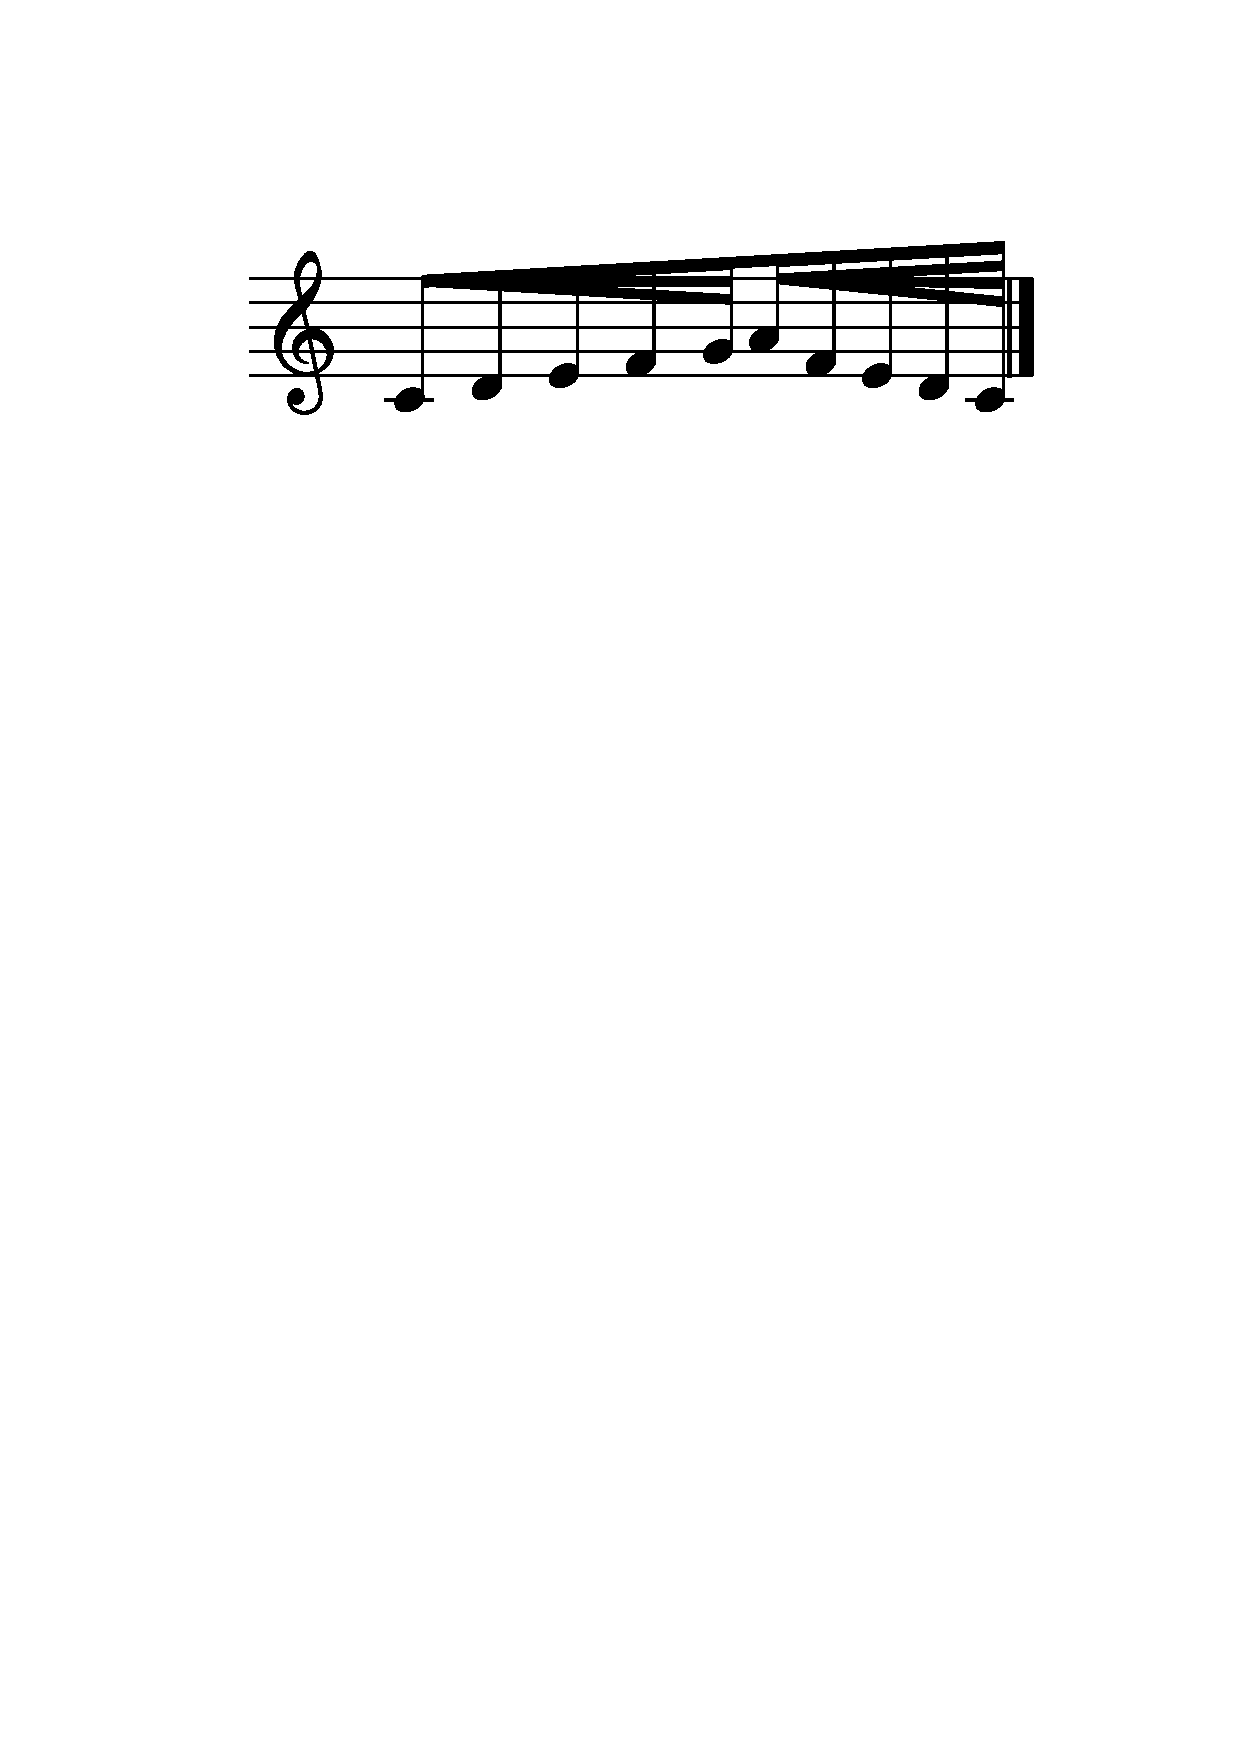
\includegraphics[width=55mm]{img/fBeamHierarchie.pdf}
\caption{\emph{Feathered beams} englobés dans un plus grand}
\label{fig:fbeamhierarchie}
\end{figure}


%*****************************EXEMPLES COMPLEXES****************************************
\subsection{Exemple de partition complexe}\label{subsec:partitionComplexe}

À l'aide des nouveaux éléments, \emph{tag} et autres implémentations effectuées dans les dernières versions, nous avons essayé de mettre en place un exemple complexe afin d'illustrer quelques nouvelles possibilités offertes par \guido.

\exemple\\
Le code suivant génère la partition présentée en figure \ref{fig:complexExemple}.
\begin{gmncode}
{
  [
    \staffFormat<style="3-line">
    \accol<id=1,range="1-2",type="straightBrace">
    \staff<id=1, dy=2.5cm>
    \barFormat<style="staff">
    \clef<"perc">
    \meter<"3+2/8"> _ _/8
    \intens<"p", dx=-1>
    \stemsUp
    \cresc<dm="ff",dx1=3,dx2=-5,dy=-1,deltaY=4>(
      \beam<dy2=0.6> (
        g/20 e g b
        g/40 e
      )
    )

    \stemsDown
    \tuplet<"-6:5-", dy1=6,dy2=10>(
      \beam<dy2=4>(
        b*5/40
        \grace(
          \stemsUp(g*5/80 b)
        )
        \accent<dy=-3>(e*5/40) _
        \tuplet<"-3-", dy1=3, dy2=5>(b*5/240 e g) 
        \accent(b*5/40)
        \grace(
          \stemsUp(g*5/80 g)
        )
        \accent<dy=-3>(e*5/80)
      )
    )
  ],
  [
    \staff<id=2>
    \staffFormat<"1-line">
    \staffOff
    \clef
    \meter<"2+3/8"> empty*5/8
    \staffOn
    \clef<"perc">
    \intens<"ff", dy=2, dx=2>
    \beam<dy2=1.5>(
      g/28
      \noteFormat<"x">(\accent(g)) g
      \noteFormat<"x">(\accent(g)) g g g
      \noteFormat<"x">(\accent(g/8))
    )
    \beam(
      g/20
      \intens<"fff", dx=-3, dy=2>
      \noteFormat<"x">(\accent(g)) g g
      \noteFormat<"x">(\accent(g))
    )
  ],
  [
    \accol<id=2, range="3-4">
    \staff<id=3, dy=1.4cm>
    \text<"gliss.", font="Times New Roman", 
      dx=35, dy=1>
    \cresc<dm="fff",dx1=2,dx2=-5,dy=3,deltaY=4>(
       \meter<"3+2/8">
       \intens<"p", dy=-4> empty/2
       \glissando(
         \noteFormat<dx=-28.5> (c/8) {
           \marcato<dy=3>(d#3), e, f#, g
         }
       )
    )
    \staffOff
  ],
  [
    \staff<id=4>
    \text<"gliss.", font="Times New Roman", 
      dx=35, dy=12>
    \meter<"3+2/8"> empty/2
    \glissando(
      \noteFormat<dx=-28.5> (b0/8) {
        \marcato<"below", dy=-5, dx=1>(a#-2), 
        g, f#, e, d
      }
    )
    \staffOff
  ]
}
\end{gmncode}

\begin{figure}[h]
\centering
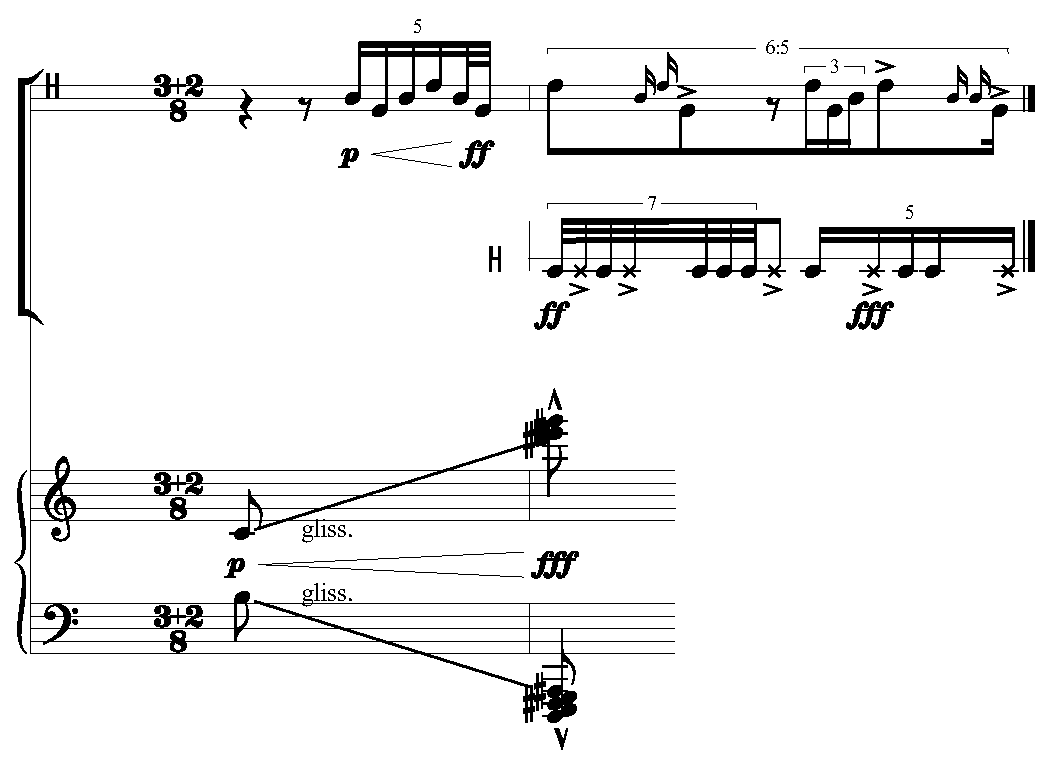
\includegraphics[width=80mm]{img/partitions/complexExemple.pdf}
\caption{Exemple de partition complexe générée avec \guido}
\label{fig:complexExemple}
\end{figure}


%*********************CONCLUSION**********************
\section{Conclusion}\label{sec:conclusion}

% a faire /////////////////////////////////////////////////////

\bibliographystyle{plain}
\bibliography{../../guido}


\end{document}

